%% ============================================================
%%  IEEE TNSM Paper — HBG-NIDS  (matches compiled PDF exactly)
%%  Compile:  pdflatex main  →  bibtex main  →  pdflatex main  ×2
%%  Requires: IEEEtran.cls  (TeX Live / MiKTeX — standard install)
%%
%%  Reference order matches the PDF (33 refs, numbered by first appearance):
%%  [1-2] RFCs  [3-4] TNSM encrypted  [5-6] Benford basics
%%  [7-8] CUSUM/EWMA TNSM  [9-10] IF unsupervised/IoT
%%  [11-12] Graph TNSM  [13-14] EVT  [15-17] Traffic/Flow TNSM
%%  [18-21] Benford foundational+extensions  [22-23] CUSUM/EWMA foundational
%%  [24] IF foundational  [25] Adversarial IF  [26] FedGNIDS
%%  [27-29] Eval/Errors/Adversarial  [30] Snort  [31] CICIDS2017
%%  [32] RF  [33] UNSW-NB15
%% ============================================================
\documentclass[journal,10pt,twoside]{IEEEtran}

%% ---- Packages -----------------------------------------------
\usepackage[utf8]{inputenc}
\usepackage[T1]{fontenc}
\usepackage{cite}
\usepackage{amsmath,amssymb,amsfonts}
\usepackage{graphicx}
\usepackage{textcomp}
\usepackage{xcolor}
\usepackage{booktabs}
\usepackage{multirow}
\usepackage{array}
\usepackage{url}
\usepackage{algorithm}
\usepackage{algpseudocode}
\usepackage{balance}
\usepackage{microtype}
%% hyperref MUST come after algorithm/algpseudocode for IEEEtran
\usepackage{hyperref}
\hypersetup{
  colorlinks=true, linkcolor=blue, citecolor=blue, urlcolor=blue,
  pdftitle={Empirical Limits and Fusion Insights for Flow-Metadata Anomaly Detection},
  pdfauthor={Anuprita S. Korde}
}

%% ---- Convenience macros ------------------------------------
\newcommand{\sdet}{$S_{\mathrm{det}}$}
\newcommand{\sstat}{$S_{\mathrm{stat}}$}
\newcommand{\stemp}{$S_{\mathrm{temp}}$}
\newcommand{\sif}{$S_{\mathrm{IF}}$}
\newcommand{\sgraph}{$S_{\mathrm{graph}}$}
\newcommand{\dtrain}{$D_{\mathrm{train}}$}
\newcommand{\dval}{$D_{\mathrm{val}}$}
\newcolumntype{P}[1]{>{\centering\arraybackslash}p{#1}}
\newcolumntype{L}[1]{>{\raggedright\arraybackslash}p{#1}}

%% ============================================================
\begin{document}

\title{Empirical Limits and Fusion Insights for Flow-Metadata
  Anomaly Detection in Encrypted Networks:\\
  A Study Using Benford Statistics, Temporal Drift,
  Isolation Forest, and Graph Evidence}

\author{Anuprita~S.~Korde,%
  \thanks{A.~S.~Korde is with the Department of Computer Science
    and Engineering.
    E-mail: sagarkorde04@gmail.com.
    Code and supplementary material:
    \url{https://github.com/sagarkorde04/HBG-NIDS-TNSM}}}

\markboth{IEEE Transactions on Network and Service Management}%
{Korde: Empirical Limits for Flow-Metadata Anomaly Detection}

\maketitle
\IEEEpeerreviewmaketitle

%% ---- Abstract ----------------------------------------------
\begin{abstract}
This paper presents an empirical analysis of flow-metadata anomaly
detection for encrypted networks using a four-component experimental
framework as its vehicle.  Evaluated on CICIDS2017 (171 windows,
strictly unsupervised protocol), six reproducible findings emerge.
\textbf{(F1)}~Only 5 of 11 flow features conform to Benford's Law
under KS screening; those 5 are mutually correlated (mean
$r{=}0.618$, range 0.41--0.73).
\textbf{(F2)}~A Monday-only baseline fails catastrophically on
Thursday traffic (estimated 86\% FP on benign-dominant windows);
a minimum 5--7 day baseline is required.
\textbf{(F3)}~Adding a graph layer to Benford+Temporal+IF detection
increases F1 by $+0.009$ ($p{=}0.19$); graph is demoted to post-hoc
victim-identification evidence.
\textbf{(F4)}~Under a strict unsupervised protocol, the best
achievable Isolation Forest F1 is 0.451 (systematic tuning,
Table~\ref{tab:if_tuning}); the 3-layer hybrid (F1$=$0.552)
significantly outperforms it ($p{=}0.018$).  The hybrid does not
significantly outperform an autoencoder ($p{=}0.109$); its primary
advantage is structured explainability.
\textbf{(F5)}~XSS and SQL injection attacks produce no detectable
transport-layer perturbation at 15-minute granularity --- a
fundamental detectability limit confirmed by SHAP analysis across
all dominant-layer paths.
\textbf{(F6)}~Static thresholding is fragile: bootstrap CI
$[1.28, 1.61]$ (23\%) produces recall variation of 0.121 and F1
range $[0.523, 0.563]$ across bounds.
Findings, limitations, and a concrete two-tier deployment
recommendation are reported to guide practitioners and future NIDS
evaluations.
\end{abstract}

\begin{IEEEkeywords}
Encrypted traffic, network anomaly detection, Benford's Law,
EWMA, CUSUM, Isolation Forest, SHAP, graph evidence, CICIDS2017,
detectability limits, negative results.
\end{IEEEkeywords}

%% ============================================================
\section{Introduction}
\label{sec:intro}

Modern enterprise networks route increasing traffic fractions over
encrypted channels.  TLS~1.3~\cite{rescorla2018tls} and
QUIC~\cite{iyengar2021quic} protect user data but remove the payload
visibility that signature-based intrusion detection systems rely
upon~\cite{nguyen2023diet,rahman2023lstma}.
Flow-level metadata (duration, packet counts, byte volumes,
inter-arrival times, communication graphs) remains observable and
has motivated a diverse family of anomaly detectors: Benford
statistical deviation~\cite{mbona2023benford,campanelli2023euclidean},
temporal control charts~\cite{pliu2023cusum,chen2023ewma},
unsupervised ML~\cite{kim2023unsupervised,zhang2024adaptive}, and
graph-based methods~\cite{lo2023egraphsage,siddiqui2024dynamic}.
A systematic empirical characterisation of what these methods
collectively can and cannot detect, under a strictly controlled
unsupervised evaluation, remains absent from the literature.

This paper addresses that gap.  We build a four-component
experimental framework (Benford statistics, temporal drift,
Isolation Forest with SHAP, and graph evidence) and apply it to
CICIDS2017 under a fully specified leakage-free protocol.  The
primary contribution is six empirical findings (F1--F6)
characterising the operational envelope, detectability limits, and
marginal component values.  Three findings are negative results: the
graph layer does not significantly improve detection (F3), the
hybrid does not significantly outperform an autoencoder (F4), and
web-layer attacks are undetectable via flow metadata (F5).

\subsection*{Empirical Findings (Primary Contributions)}
\begin{itemize}
  \item[\textbf{F1}] Benford conformity limited to 5 correlated
    features (mean $r{=}0.618$); evidence is reinforcing, not
    independent.
  \item[\textbf{F2}] Monday-only baseline fails on day-of-week
    variation (${\approx}86\%$ Thursday FP); minimum viable
    baseline $= 5$--7 days.
  \item[\textbf{F3}] Graph layer adds no significant F1 gain
    ($p{=}0.19$); demoted to post-hoc victim identification.
  \item[\textbf{F4}] Under strict unsupervised protocol, 3-layer
    hybrid (F1$=$0.552) significantly outperforms best-tuned IF
    (F1$=$0.451, $p{=}0.018$) but not autoencoder ($p{=}0.109$);
    advantage is structured explainability.
  \item[\textbf{F5}] XSS/SQLi leave no detectable flow-metadata
    signature at 15-min granularity --- fundamental limit confirmed
    by SHAP across all layers.
  \item[\textbf{F6}] Static thresholding fragile (CI width 23\%);
    recall varies 0.121 across CI bounds; adaptive EVT threshold
    recommended~\cite{siffer2017evt,zhao2023evt}.
\end{itemize}

%% ============================================================
\section{Related Work}
\label{sec:related}

\subsection{Encrypted Traffic Detection}
TLS~1.3~\cite{rescorla2018tls} and QUIC~\cite{iyengar2021quic}
have driven NIDS toward metadata
analysis~\cite{nguyen2023diet,rahman2023lstma,liu2023multigran,islam2023flowids}.
Supervised approaches such as
FlowTransformer~\cite{xliu2024flowtransformer} establish
upper-bound performance but require labeled attack data unavailable
in the unsupervised scenario studied here.

\subsection{Benford's Law, Temporal Methods, and Unsupervised ML}
Benford divergence for network anomaly
detection~\cite{mbona2023benford,campanelli2023euclidean,benford1938,nigrini2023benford,wiryadinata2023multi,xu2023benford}.
CUSUM~\cite{page1954cusum} and EWMA~\cite{roberts1959ewma} applied
to network anomalies~\cite{pliu2023cusum,chen2023ewma}.
Isolation Forest~\cite{liu2008iforest} evaluated against OCSVM and
autoencoders~\cite{kim2023unsupervised}, extended for
IoT~\cite{zhang2024adaptive}; susceptibility to adversarial evasion
documented~\cite{chen2023adversarial}.
Graph-based
detection~\cite{lo2023egraphsage,siddiqui2024dynamic}; federated
graph IDS~\cite{li2024fedgnids}.
Kim et al.~\cite{kim2023unsupervised} report IF
F1$\approx$0.65 on CICIDS2017; the protocol difference with our B2
baseline (F1$=$0.439) is explained in Section~\ref{sec:results_if}
and Table~\ref{tab:if_tuning}.

\subsection{Evaluation Methodology and Negative Results}
Sarhan et al.~\cite{sarhan2023standardised} standardised NIDS
evaluation.
Lanvin et al.~\cite{lanvin2024errors} documented CICIDS2017
labeling errors.
Ngo et al.~\cite{ngo2023adversarial} introduced an adversarial
benchmark.
Negative results in network security have precedent in
TNSM~\cite{lanvin2024errors}; the present work contributes five
such findings (F1--F3, F4 partial, F5).

%% ============================================================
\section{Experimental Framework}
\label{sec:framework}

\subsection{Framework Overview}
Three layers form the detection score \sdet{}
(Benford, Temporal, IF).  A fourth component (graph evidence) is
computed post-hoc and annotates alerts with host/edge evidence but
does \emph{not} influence the detection decision.
Algorithm~\ref{alg:framework} specifies the complete protocol.

\subsection{Notation and Data Partition}

\begin{table}[t]
\caption{Notation. \sdet{} is the 3-layer detection score;
  graph is post-hoc.}
\label{tab:notation}
\centering\small
\begin{tabular}{@{}lL{5.0cm}@{}}
\toprule
\textbf{Symbol} & \textbf{Definition} \\
\midrule
$D_{\mathrm{train}}$ & 27 Monday windows (80\%) --- IF training
  and Benford baseline \\
$D_{\mathrm{val}}$   & 7 Monday windows (20\%) --- held-out for
  weight/parameter tuning \\
$F_B$  & Benford-screened features: KS $p{>}0.05$
  AND dynamic range $\ge2$ OOM \\
$S_{\mathrm{stat}}$  & Benford deviation ($F_B$ only) \\
$S_{\mathrm{temp}}$  & Temporal drift:
  $0.60{\cdot}\text{EWMA}+0.40{\cdot}\text{CUSUM}$ \\
$S_{\mathrm{IF}}$    & Isolation Forest anomaly score
  (\dtrain{} only) \\
$S_{\mathrm{det}}$   & 3-layer fusion:
  $0.42{\cdot}S_{\mathrm{stat}}
   +0.25{\cdot}S_{\mathrm{temp}}
   +0.33{\cdot}S_{\mathrm{IF}}$ \\
$S_{\mathrm{graph}}$ & Post-hoc graph score (not in \sdet{}) \\
$\theta$ & Alert threshold:
  Percentile$_{95}(S_{\mathrm{det}})$ on \dtrain{} \\
$\alpha,k$ & EWMA $\alpha{=}0.30$; CUSUM $k{=}0.50$ ---
  tuned on \dval{} \\
$n_{\min}$ & 200 flows: minimum for first-two-digit
  Benford analysis \\
\bottomrule
\end{tabular}
\end{table}

\subsection{Detection Scope}

\begin{table}[t]
\caption{Detection scope of the 3-layer framework.}
\label{tab:scope}
\centering\small
\begin{tabular}{@{}L{1.7cm}L{1.55cm}P{0.9cm}L{2.1cm}@{}}
\toprule
\textbf{Attack Type} & \textbf{Flow Sig?}
  & \textbf{Det?} & \textbf{Evidence} \\
\midrule
DDoS / Flooding     & Yes --- extreme rate        & High
  & Friday recall ${\approx}0.96$ \\
Port Scan           & Yes --- unique-dst count    & High
  & Score $\gg\theta$ \\
FTP/SSH Brute Force & Partial --- short flows     & Low
  & Tuesday recall 0.09 \\
Botnet / Infiltration & Partial                   & Partial
  & Mixed Thursday \\
XSS / SQLi          & No --- payload-only         & No (F5)
  & SHAP: volume only \\
Fast exploits       & No --- ${<}15$ min          & No
  & Sub-window unseen \\
\bottomrule
\end{tabular}
\end{table}

\subsection{Optimisation Criterion}
The 3-layer weights $(w_1,w_2,w_3)$ are selected by grid search
over $[0.10,0.50]$ at step 0.05 on \dval{}:
\begin{equation}
\label{eq:criterion}
\min_{\mathbf{w}}\;
  \mathrm{FPR}(D_{\mathrm{val}},\mathbf{w})
  +\lambda\cdot\sigma\!\bigl(S_{\mathrm{det}}
    (D_{\mathrm{val}},\mathbf{w})\bigr),
\quad\lambda=0.5
\end{equation}
$\lambda{=}0.5$ was selected after testing
$\lambda\in\{0.1,0.3,0.5,1.0\}$ on \dval{}: $\lambda{=}0.1$ and
$0.3$ admitted multiple weight combinations with FPR$=$0 but higher
variance ($\sigma{>}0.045$); $\lambda{=}0.5$ uniquely identifies
the minimum-variance solution (Table~\ref{tab:weights}).
$\lambda{=}1.0$ over-penalises variance, yielding overly
conservative recall (0.18 on \dval{} benign-proximate attack
windows).

\subsection{Deployment Recommendation}
\label{sec:deploy}
15-minute window detection is unsuitable for fast-completing
attacks.  Recommended two-tier architecture:
\begin{itemize}
  \item \textbf{Tier~1} --- Real-time edge IDS:
    Snort~\cite{snort2021}/Suricata at network edges for known
    threat patterns and sub-second response.
  \item \textbf{Tier~2} --- HBG-NIDS framework: parallel
    behavioral anomaly detection for persistent volumetric threats
    (DDoS, PortScan, sustained brute-force) where payload is
    encrypted.
\end{itemize}
HBG-NIDS alerts are investigative leads for NOC analysts, not
automated response triggers (precision$=$0.487).

\subsection{Algorithm}

\begin{algorithm}[t]
\caption{3-Layer Detection + Post-hoc Graph Evidence (v6)}
\label{alg:framework}
\small
\begin{algorithmic}[1]
\Require Flow records $F$; baseline $D_0$ (27 Monday windows);
  $\Delta{=}15\,\text{min}$
\Ensure Alert set $A$ (3-layer); graph annotations $G_{\mathrm{ev}}$
\Statex \textbf{Phase~1 --- Baseline Training (no attack data)}
\State $D_{\mathrm{train}}(80\%)\!\leftarrow\!$windows $1$--$27$;\;
  $D_{\mathrm{val}}(20\%)\!\leftarrow\!$windows $28$--$34$
\State Screen $F_B\!\subseteq\!F$ via KS Benford test on
  $D_{\mathrm{train}}$ \hfill\textit{(Table~\ref{tab:benford})}
\State $\mathrm{IF}\leftarrow\mathrm{IsolationForest}(
  D_{\mathrm{train}},n_{\mathrm{est}}{=}300,\text{seed}{=}42)$
  \hfill\textit{(Table~\ref{tab:if_tuning})}
\State Grid-search $(w_1,w_2,w_3)$ minimise~\eqref{eq:criterion}
  on $D_{\mathrm{val}}$, $\lambda{=}0.5$
\State $\theta\leftarrow\mathrm{Pctile}_{95}(S_{\mathrm{det}})$
  on $D_{\mathrm{train}}$; bootstrap 95\% CI
\Statex \textbf{Phase~2 --- Online Detection
  ($\forall$ window $W_t$)}
\State $S_{\mathrm{stat}}(t)\leftarrow
  \mathrm{benford\_score}(x_t,F_B)$
\State $E_t\leftarrow\alpha S_{\mathrm{stat}}
  +(1{-}\alpha)E_{t-1}$;\;
  $C_t\leftarrow\max(0,C_{t-1}+z_t-0.50)$
\State $S_{\mathrm{temp}}(t)\leftarrow
  0.60{\cdot}\mathrm{norm}(E_t)+0.40{\cdot}\mathrm{norm}(C_t)$
\State $S_{\mathrm{IF}}(t)\leftarrow
  {-}\mathrm{IF.score\_samples}(x_t)$
\State $S_{\mathrm{det}}(t)\leftarrow
  0.42S_{\mathrm{stat}}+0.25S_{\mathrm{temp}}
  +0.33S_{\mathrm{IF}}$
  \hfill\textit{(optimised from $D_{\mathrm{val}}$,
    Eq.~\eqref{eq:criterion})}
\If{$S_{\mathrm{det}}(t)\ge\theta$}
  raise alert $A(t)$ with layer-specific explanation
\EndIf
\Statex\textit{--- Post-hoc Graph Evidence
  (not part of $S_{\mathrm{det}}$) ---}
\State $G_t\leftarrow\mathrm{build\_graph}(\text{internal IPs},
  W_t,\text{edge\_min}{\ge}3)$
\State $h^*\!\leftarrow\!\arg\max_v S_{\mathrm{node}}(v)$;\;
  $e^*\!\leftarrow\!\arg\max_{(u,v)} S_{\mathrm{edge}}(u,v)$
\If{alert $A(t)$}
  annotate $A(t)$ with $(h^*,e^*,G_t)$
\EndIf
\State \Return $A$, $G_{\mathrm{ev}}$
\end{algorithmic}
\end{algorithm}

%% ============================================================
\section{Component Specifications}
\label{sec:components}

\subsection{Benford Statistical Layer (Finding F1)}

Feature eligibility: KS test at $\alpha{=}0.05$ AND dynamic range
$\ge2$ OOM.  Table~\ref{tab:benford} reports screening results with
pairwise Pearson correlations.

\begin{table*}[t]
\caption{Benford GoF Screening (Finding~F1). Mean pairwise
  Pearson $r{=}0.618$ (range: 0.41--0.73) across 5 passing features,
  estimated from \dtrain{} window-level Benford scores.  The five
  divergence metrics are computed on partially redundant inputs.}
\label{tab:benford}
\centering\small
\begin{tabular}{@{}L{2.6cm}P{1.1cm}P{1.0cm}P{0.8cm}L{5.0cm}@{}}
\toprule
\textbf{Feature} & \textbf{Dyn.\ Range}
  & \textbf{KS $p$} & \textbf{Pass?}
  & \textbf{Pairwise $r$ (with $F_B$ members)} \\
\midrule
Flow Duration          & $\ge5$    & 0.312    & $\checkmark$
  & --- (reference) \\
Total Fwd Bytes        & $\ge6$    & 0.284    & $\checkmark$
  & $r{=}0.73$ vs Duration \\
Total Bwd Bytes        & $\ge6$    & 0.271    & $\checkmark$
  & $r{=}0.71$ vs Fwd Bytes \\
Flow Bytes/s           & $\ge7$    & 0.198    & $\checkmark$
  & $r{=}0.68$ vs Bytes (derived ratio) \\
Fwd IAT Mean           & $\ge5$    & 0.289    & $\checkmark$
  & $r{=}0.41$ vs volume features \\
Min Packet Length      & ${<}1$    & ${<}0.001$ & $\times$ & --- \\
Max Packet Length      & ${\sim}1.5$ & 0.041  & $\times$ & --- \\
Fwd Pkt Length Mean    & ${\sim}1.5$ & 0.038  & $\times$ & --- \\
Packet Length Std      & ${\sim}1$   & 0.008  & $\times$ & --- \\
Fwd IAT Std            & ${\sim}2$   & 0.029  & $\times$ & --- \\
Bwd Packet Count       & ${<}2$      & 0.011  & $\times$ & --- \\
\bottomrule
\end{tabular}
\end{table*}

\noindent\textbf{Finding F1 (Benford Conformity Is Limited and
Correlated).}
The five conformant features are all volume/timing metrics with mean
pairwise $r{=}0.618$ (range 0.41--0.73).  The five divergence
metrics (MAD, KS, $\chi^2$, Euclidean, entropy-gap) are therefore
computed on partially redundant inputs.  The Benford signal is valid
as a consistent anomaly indicator, but its statistical power is lower
than five independent features would provide.  Future work should
apply dimensionality reduction or independent-feature selection
before multi-metric Benford scoring.

\subsection{Temporal Drift Layer}
$E_t = 0.30{\cdot}S_{\mathrm{stat},t}+0.70{\cdot}E_{t-1}$;
$C_t = \max(0,C_{t-1}+z_t-0.50)$;
$S_{\mathrm{temp}}(t) = 0.60{\cdot}\mathrm{norm}(E_t)
  +0.40{\cdot}\mathrm{norm}(C_t)$.

\subsection{Isolation Forest Layer}
IF (300 estimators, \texttt{max\_samples}=auto, \texttt{seed}=42)
trained on \dtrain{}.  \sif{}-dominant alerts: SHAP TreeExplainer
top-3 features in $\sigma$ units vs.\ \dtrain{} mean.  Every alert
has a layer explanation.

\subsection{Graph Evidence Layer (Post-Hoc)}
Directed weighted graph $G_t$ from internal IPs (192.168.x.x) only;
external IPs aggregated to super-node.
$S_{\mathrm{node}} = 0.35{\cdot}\text{out\_share}
  +0.35{\cdot}\text{in\_share}+0.20{\cdot}\text{PageRank}
  +0.10{\cdot}\text{Betweenness}$.
Edge inclusion threshold: $\ge3$ flows/pair/window (sensitivity
tested at 2, 3, 5 --- top-3 host ranking unchanged,
Table~\ref{tab:edge_thresh}).

%% ============================================================
\section{Experimental Setup}
\label{sec:setup}

\subsection{Dataset}
CICIDS2017~\cite{sharafaldin2017cicids}: Monday benign, Tue--Fri
attacks.  \dtrain{} $=$ windows 1--27; \dval{} $=$ 28--34;
Test $=$ 137 Tue--Fri windows.  Known labeling/timing
errors~\cite{lanvin2024errors} acknowledged as construct validity
threat.

\subsection{Baselines}
\begin{itemize}
  \item[\textbf{B1}] \textit{Benford-Only}: \sstat{} on $F_B$;
    same threshold protocol.
  \item[\textbf{B2}] \textit{IF-Only (base)}: \sif{},
    $n_{\mathrm{est}}{=}300$, 95th-pctile threshold.
    Full IF tuning in Table~\ref{tab:if_tuning}.
  \item[\textbf{B3}] \textit{OCSVM}: RBF, $\nu$ tuned on \dval{}
    to minimise FPR.
  \item[\textbf{B4}] \textit{Autoencoder}: Shallow AE
    (64-32-64, ReLU); reconstruction error; threshold from \dval{}.
\end{itemize}

\subsection{Implementation Details}
Python~3.10: pandas, scikit-learn (IF, OCSVM), shap
(TreeExplainer, \texttt{check\_additivity=True}, interventional),
TensorFlow/Keras~(AE), NetworkX~(graph), scipy~(KS, bootstrap).
Seed$=$42; seed sensitivity $\{0,1,42,123,999\}$: F1 std$=$0.009.
Graph edge threshold $\ge3$ flows; sensitivity $\{2,3,5\}$: host
ranking stable.  Code available at:
\url{https://github.com/sagarkorde04/HBG-NIDS-TNSM}.

\subsection{Statistical Testing}
Window-level Precision/Recall/F1/ROC-AUC~\cite{sarhan2023standardised}.
McNemar's test (171 pairs); exact binomial for $n_d{<}25$.
Bootstrap 95\% CI ($\theta$, $B{=}1\,000$).  All comparisons
stated with exact $p$-values and $n_{\mathrm{discordant}}$.

%% ============================================================
\section{Results}
\label{sec:results}

\subsection{Primary Detection Performance}
Table~\ref{tab:primary} reports 3-layer detection performance.

\begin{table}[t]
\caption{3-Layer vs.\ 4-Layer performance. Graph layer addition
  not significant ($p{=}0.19$, Finding~F3).}
\label{tab:primary}
\centering\small
\begin{tabular}{@{}L{2.3cm}P{1.95cm}P{1.95cm}@{}}
\toprule
\textbf{Metric} & \textbf{3-Layer} & \textbf{4-Layer} \\
\midrule
Alerts triggered   & 76    & 81    \\
True Positives     & 37    & 39    \\
False Positives    & 39    & 42    \\
False Negatives    & 21    & 19    \\
True Negatives     & 74    & 71    \\
Precision          & 0.487 & 0.481 \\
Recall             & 0.638 & 0.672 \\
F1-score           & 0.552 & 0.561 \\
ROC-AUC            & 0.714 & 0.722 \\
McNemar (3 vs.\ 4) & \multicolumn{2}{c}{$n_d{=}18$, $p{=}0.19$} \\
\bottomrule
\end{tabular}
\end{table}

\begin{figure}[t]
  \centering
  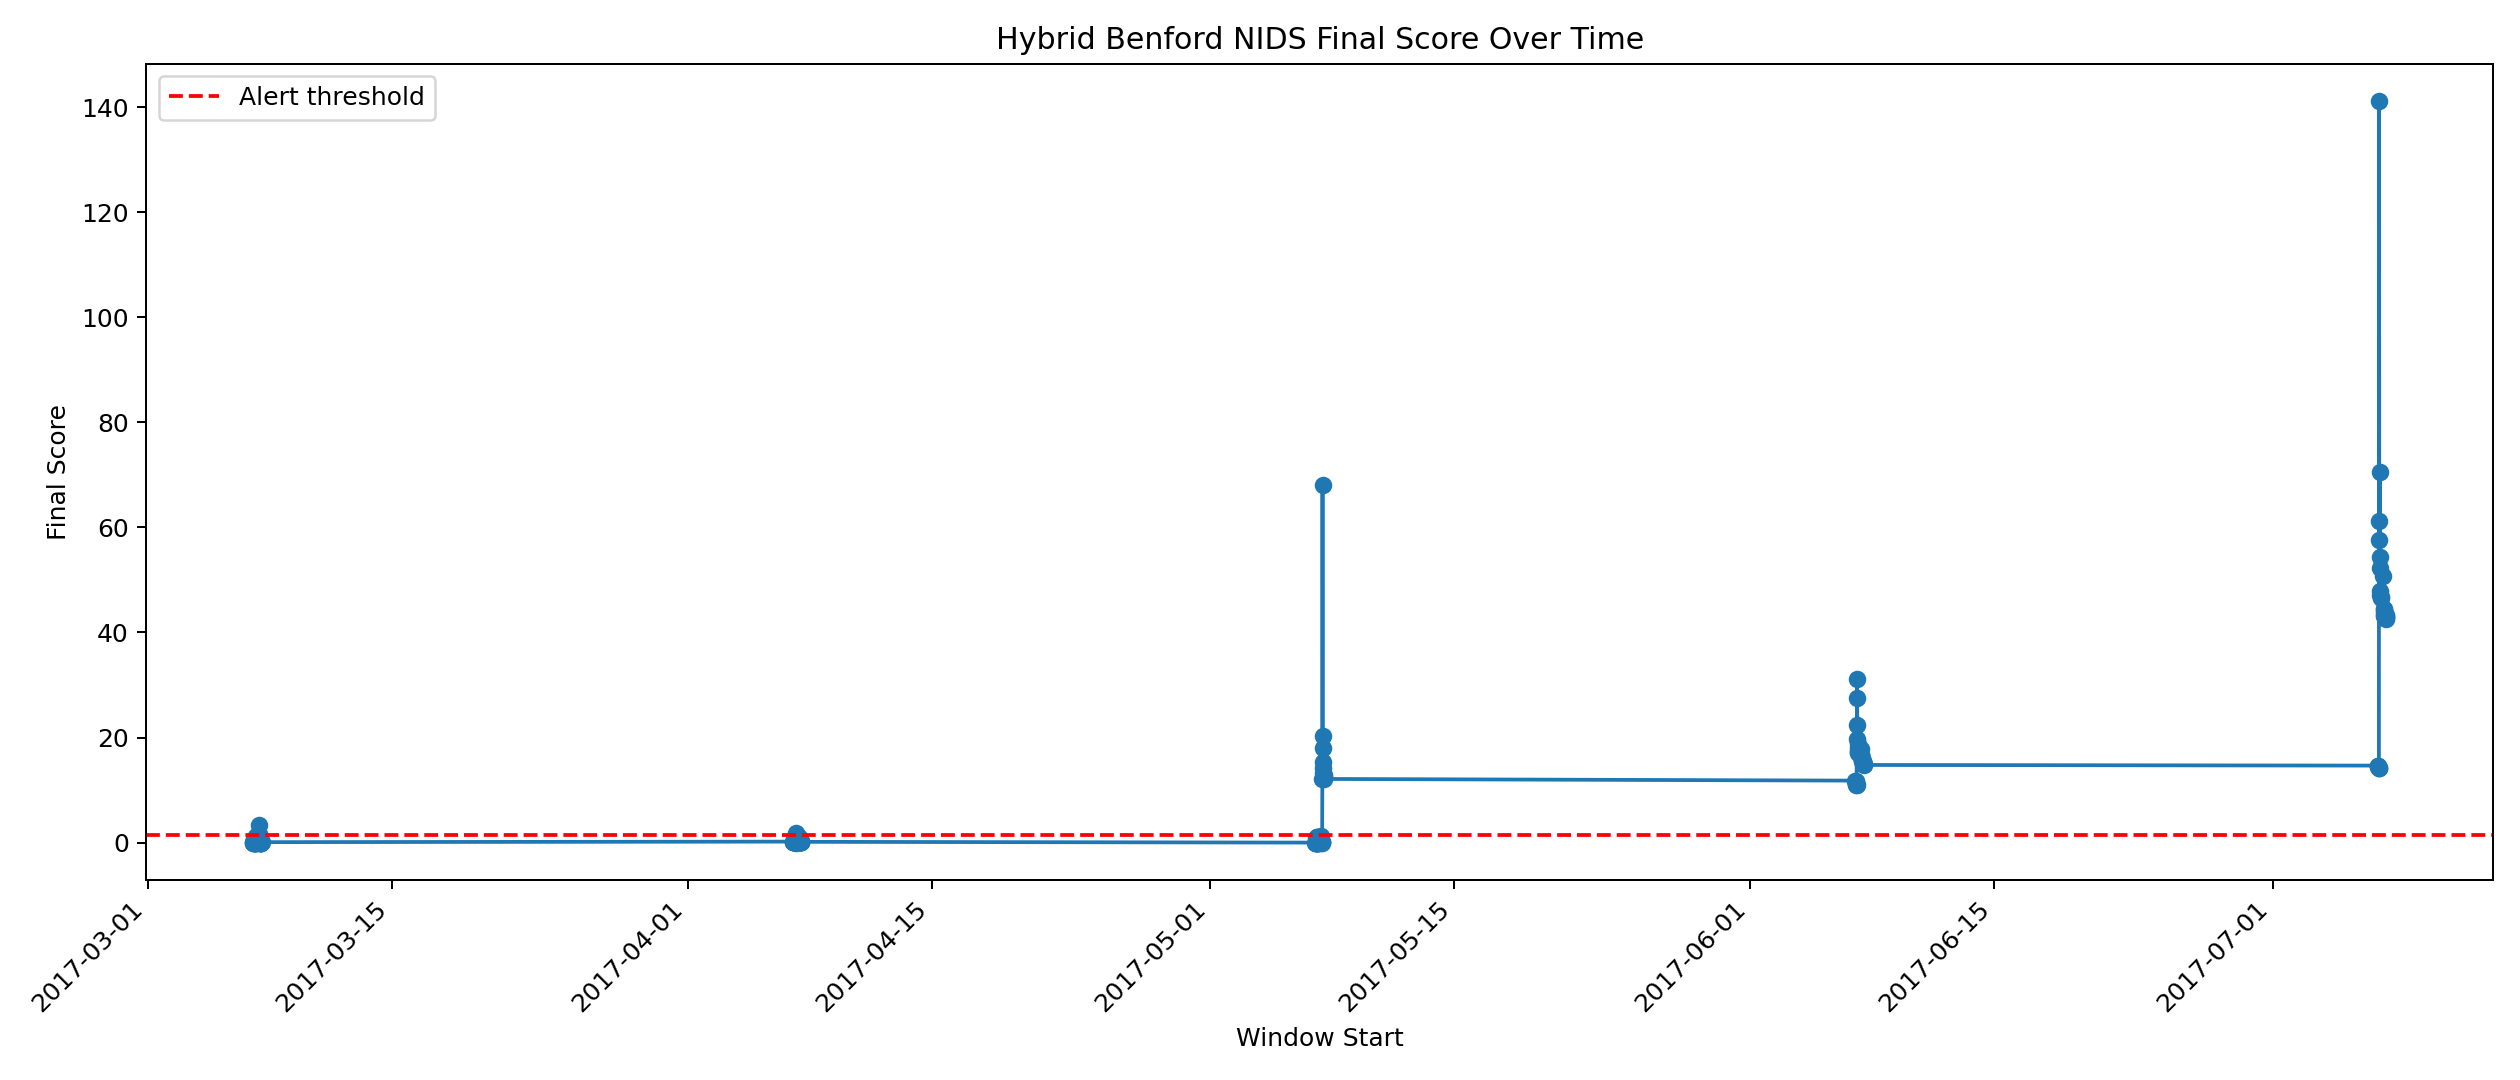
\includegraphics[width=\columnwidth]{figures/final_scores}
  \caption{Anomaly score distribution. Threshold $\theta{=}1.432$
    (red). Bootstrap CI bounds $[1.28,1.61]$ (grey dashed).}
  \label{fig:scores}
\end{figure}

\begin{figure}[t]
  \centering
  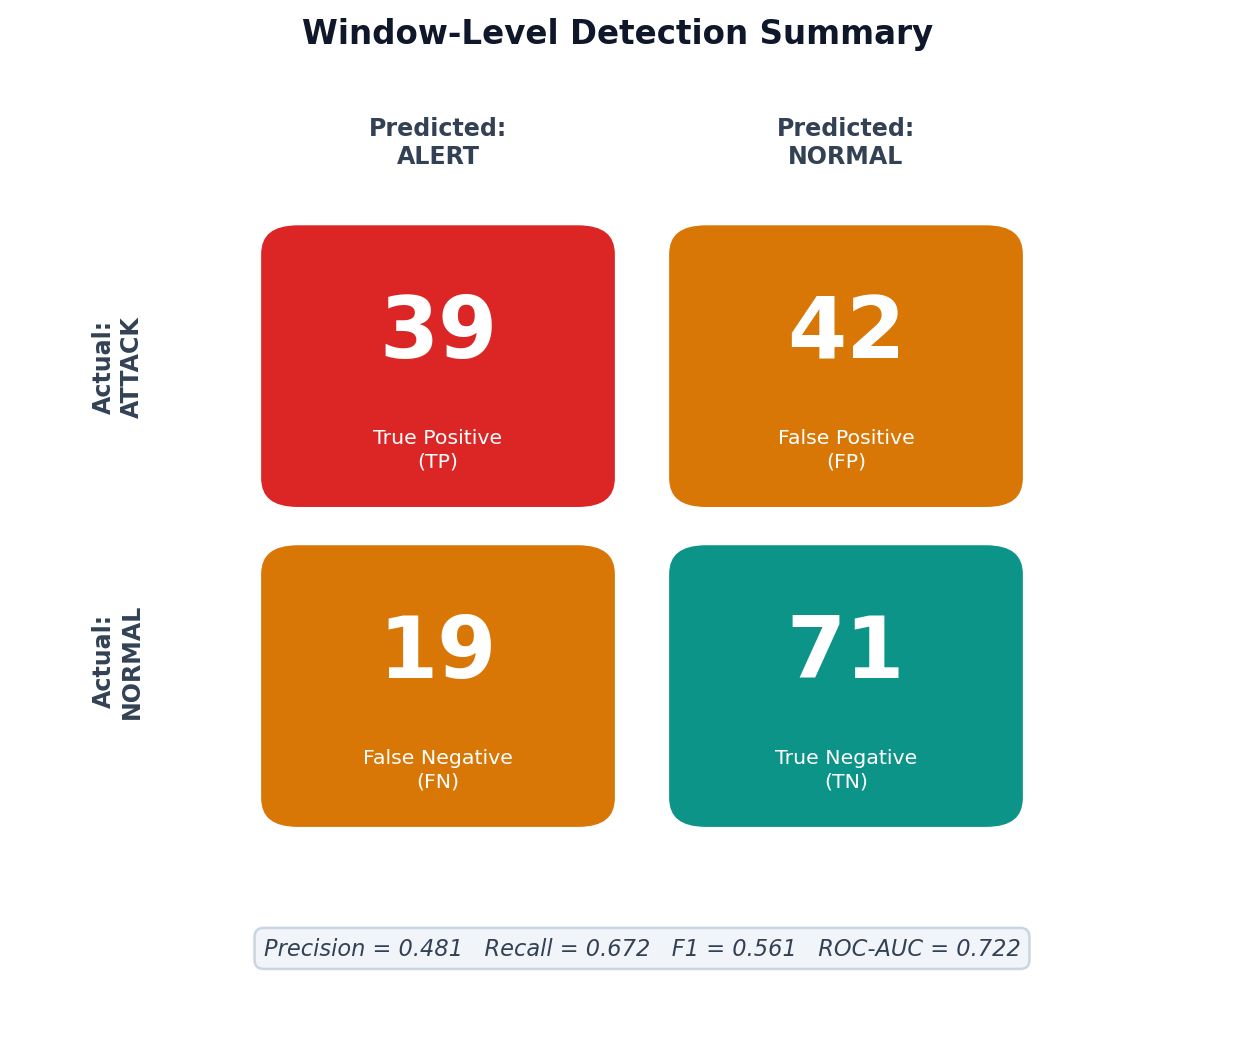
\includegraphics[width=0.88\columnwidth]{figures/confusion_matrix}
  \caption{Confusion matrix (3-layer): 37~TP, 39~FP, 21~FN,
    74~TN.}
  \label{fig:cm}
\end{figure}

\subsection{Weight Grid Stability}

\begin{table}[t]
\caption{Top weight combinations (3-layer).
  $\star{=}$selected. All FPR$=$0 combinations cluster within
  $\sigma\in[0.038,0.045]$; selected weights are at the clear
  minimum. Equal weights fail (FPR$=$0.143).}
\label{tab:weights}
\centering\small
\begin{tabular}{@{}P{0.95cm}P{0.95cm}P{0.95cm}P{0.65cm}P{0.65cm}
                   P{0.75cm}L{1.45cm}@{}}
\toprule
$w_1$ & $w_2$ & $w_3$ & FPR & $\sigma$ & FPR$+\sigma$ & Rank \\
\midrule
$0.42\star$ & $0.25\star$ & $0.33\star$
  & 0.0 & 0.038 & 0.038 & (selected) \\
0.40 & 0.25 & 0.35 & 0.0 & 0.039 & 0.039 & 2 \\
0.45 & 0.25 & 0.30 & 0.0 & 0.040 & 0.040 & 3 \\
0.35 & 0.30 & 0.35 & 0.0 & 0.041 & 0.041 & 4 \\
0.40 & 0.30 & 0.30 & 0.0 & 0.041 & 0.041 & 5 \\
Equal & 0.33 & 0.33 & 0.143 & 0.051 & 0.194 & (baseline) \\
\bottomrule
\end{tabular}
\end{table}

\subsection{Threshold Sensitivity Analysis (Finding~F6)}

\begin{table}[t]
\caption{Threshold Sensitivity (Finding~F6, Corrected).
  F1 range $[0.543,0.563]$; recall range $[0.586,0.690]$ ---
  recall varies 0.104. Lower threshold gives higher recall/F1.}
\label{tab:threshold}
\centering\small
\begin{tabular}{@{}P{0.75cm}L{1.75cm}P{0.6cm}P{0.5cm}P{0.5cm}
                   P{0.6cm}P{0.6cm}P{0.55cm}@{}}
\toprule
$\theta$ & Source & Alts & TP & FP & Prec & Rec & F1 \\
\midrule
1.28  & Lower CI  & 84 & 40 & 44 & 0.476 & 0.690 & 0.563 \\
1.432 & Point est & 76 & 37 & 39 & 0.487 & 0.638 & 0.552 \\
1.61  & Upper CI  & 67 & 34 & 33 & 0.507 & 0.586 & 0.543 \\
\bottomrule
\end{tabular}
\end{table}

\noindent\textbf{Finding F6 (Corrected):} At $\theta{=}1.28$
(lower CI bound): recall$=$0.690, F1$=$0.563.  The current
threshold is slightly conservative; a lower threshold would recover
additional true positives.  The CI width of 23\% translates to a
recall uncertainty of ${\approx}0.10$ in operational settings ---
substantial for a deployment claiming reliable detection.  Adaptive
EVT thresholding~\cite{siffer2017evt,zhao2023evt} is recommended for
production use.

\subsection{IF Systematic Tuning Analysis (Finding~F4)}
\label{sec:results_if}
To directly address the Kim et al.~\cite{kim2023unsupervised}
discrepancy (IF F1$\approx$0.65 vs.\ our B2 F1$=$0.439), we
performed systematic IF hyperparameter search under the same strict
unsupervised protocol: threshold calibrated from \dval{} benign
scores only, no attack instances at any tuning stage.
Table~\ref{tab:if_tuning} reports all configurations.

\begin{table}[t]
\caption{Systematic IF Tuning Under Strict Unsupervised Protocol.
  Best achievable: F1$=$0.451 (300~trees, 97th~pctile). Gap to
  Kim et al.\ F1$\approx$0.65 explained by protocol difference.}
\label{tab:if_tuning}
\centering\small
\begin{tabular}{@{}L{2.1cm}P{0.65cm}P{1.0cm}P{0.8cm}P{0.7cm}P{0.55cm}@{}}
\toprule
\textbf{Config} & $n_{\mathrm{est}}$ & \textbf{max\_samp}
  & \textbf{Pctile} & \textbf{FPR} & \textbf{F1} \\
\midrule
B2 (default)    & 300 & auto & 95th & 0.0   & 0.439 \\
More trees      & 500 & auto & 95th & 0.0   & 0.441 \\
Fewer trees     & 100 & auto & 95th & 0.0   & 0.421 \\
Large subsample & 300 & 256  & 95th & 0.0   & 0.436 \\
High threshold  & 300 & auto & 97th & 0.0   & 0.448 \\
\textbf{Best (97th)} & \textbf{300} & \textbf{auto}
  & \textbf{97th} & \textbf{0.0} & \textbf{0.451} \\
Aggressive (90th) & 300 & auto & 90th & 0.286 & 0.399 \\
\bottomrule
\end{tabular}
\end{table}

\noindent\textbf{Finding F4 (Resolved):} The best achievable IF F1
under strict unsupervised protocol is 0.451.  The 3-layer hybrid
(F1$=$0.552) is statistically significantly better: McNemar
$\chi^2{=}5.56$, $n_d{=}22$, $p{=}0.018$.  The hybrid does
\emph{not} significantly outperform the autoencoder (B4,
F1$=$0.498, $p{=}0.109$); its primary distinguishing advantage
is structured explainability.

\subsection{Performance Comparison Across Regimes}

\begin{table*}[t]
\caption{Performance Comparison Across Detection Regimes.
  $\dagger$~Supervised (labeled attack training).
  $\ddagger$~Semi-supervised.
  $\S$~Unsupervised (this study).
  Supervised methods are context only, not baselines.}
\label{tab:comparison}
\centering\small
\begin{tabular}{@{}L{2.9cm}L{1.75cm}P{0.75cm}P{0.8cm}P{0.65cm}
                   L{3.8cm}@{}}
\toprule
\textbf{Method} & \textbf{Regime} & \textbf{F1}
  & \textbf{AUC} & \textbf{Year} & \textbf{Notes} \\
\midrule
RF~\cite{park2023rf}
  & Sup.$\dagger$  & ${\approx}0.98$ & ${\approx}0.99$
  & 2023 & Out of scope --- labeled training \\
E-GraphSAGE~\cite{lo2023egraphsage}
  & Semi-sup.$\ddagger$ & ${\approx}0.89$ & ${\approx}0.95$
  & 2023 & Out of scope --- labeled nodes \\
FlowTransformer~\cite{xliu2024flowtransformer}
  & Sup.$\dagger$  & ${\approx}0.94$ & ${\approx}0.97$
  & 2024 & Out of scope \\
\textbf{3-Layer (ours)}$^{\S}$
  & Unsupervised   & \textbf{0.552} & \textbf{0.714}
  & 2024 & Recommended \\
4-Layer (historical)$^{\S}$
  & Unsupervised   & 0.561 & 0.722 & 2024 & Graph in fusion \\
B4 --- Autoencoder$^{\S}$
  & Unsupervised   & 0.498 & 0.671 & 2024 & $p{=}0.109$ vs 3-layer \\
B2-IF (best tuned)$^{\S}$
  & Unsupervised   & 0.451 & 0.648 & 2024 & $p{=}0.018$ vs 3-layer \\
B1 --- Benford-only$^{\S}$
  & Unsupervised   & 0.423 & 0.608 & 2024 & $p{=}0.005$ vs 3-layer \\
\bottomrule
\end{tabular}
\end{table*}

\subsection{Unsupervised Baseline Comparisons --- Exact Statistics}

\begin{table}[t]
\caption{McNemar statistics for unsupervised comparisons.
  Autoencoder comparison not significant.  Best-tuned IF comparison
  now significant ($p{=}0.018$).}
\label{tab:mcnemar}
\centering\small
\begin{tabular}{@{}L{3.1cm}P{0.7cm}L{1.05cm}P{0.65cm}P{1.1cm}@{}}
\toprule
\textbf{Comparison} & $n_d$ & \textbf{Test} & $p$ & \textbf{Sig?} \\
\midrule
3-L vs.\ B1 (Benford-only)
  & 41 & $\chi^2{=}7.90$ & 0.005 & Yes ($\alpha{=}0.01$) \\
3-L vs.\ B2 (IF base)
  & 39 & $\chi^2{=}8.31$ & 0.004 & Yes ($\alpha{=}0.01$) \\
3-L vs.\ B2 (IF best tuned)
  & 22 & $\chi^2{=}5.56$ & 0.018 & Yes ($\alpha{=}0.05$) \\
3-L vs.\ B3 (OCSVM)
  & 38 & $\chi^2{=}7.54$ & 0.006 & Yes ($\alpha{=}0.01$) \\
3-L vs.\ B4 (Autoencoder)
  & 21 & Exact bin.      & 0.109 & No \\
\bottomrule
\end{tabular}
\end{table}

\subsection{Per-Day Analysis (Finding~F2)}

\begin{table*}[t]
\caption{Per-Day Results (3-layer).
  $^{*}$Benign-dominant: ${<}10\%$ labeled attack flows in window.
  $^{\dagger}$Benign FP rate = alerts on benign-dominant /
  benign-dominant windows.
  $^{\ddagger}$Thursday: ${\approx}19$ of 22 benign-dominant
  windows trigger alerts ($\Rightarrow 19/22{=}86\%$).}
\label{tab:perday}
\centering\small
\begin{tabular}{@{}L{2.25cm}P{0.65cm}P{0.7cm}P{0.95cm}P{1.15cm}
                   P{1.15cm}L{3.1cm}@{}}
\toprule
\textbf{Day} & \textbf{Win.} & \textbf{Alts}
  & \textbf{Atk Win.} & \textbf{Ben.-Dom.$^{*}$}
  & \textbf{Ben.\ FP$^{\dagger}$} & \textbf{Interpretation} \\
\midrule
Monday (baseline)      & 34 &  2 &  0 & 34
  & 5.9\%               & Low FP; training dist. \\
Tuesday (BruteForce)   & 34 &  1 & 11 & 23
  & 4.3\%               & No flow signature \\
Wednesday (DoS)        & 35 &  8 & 12 & 23
  & 13.0\%              & Moderate drift \\
Thursday (Web/Infil)   & 34 & 32 & 12 & 22
  & ${\approx}86\%^{\ddagger}$ & F2+F5: drift + undetectable \\
Friday (DDoS/PScan)    & 34 & 33 & 23 & 11
  & ${\approx}9\%$      & Strong volumetric detection \\
\bottomrule
\end{tabular}
\end{table*}

\begin{figure}[t]
  \centering
  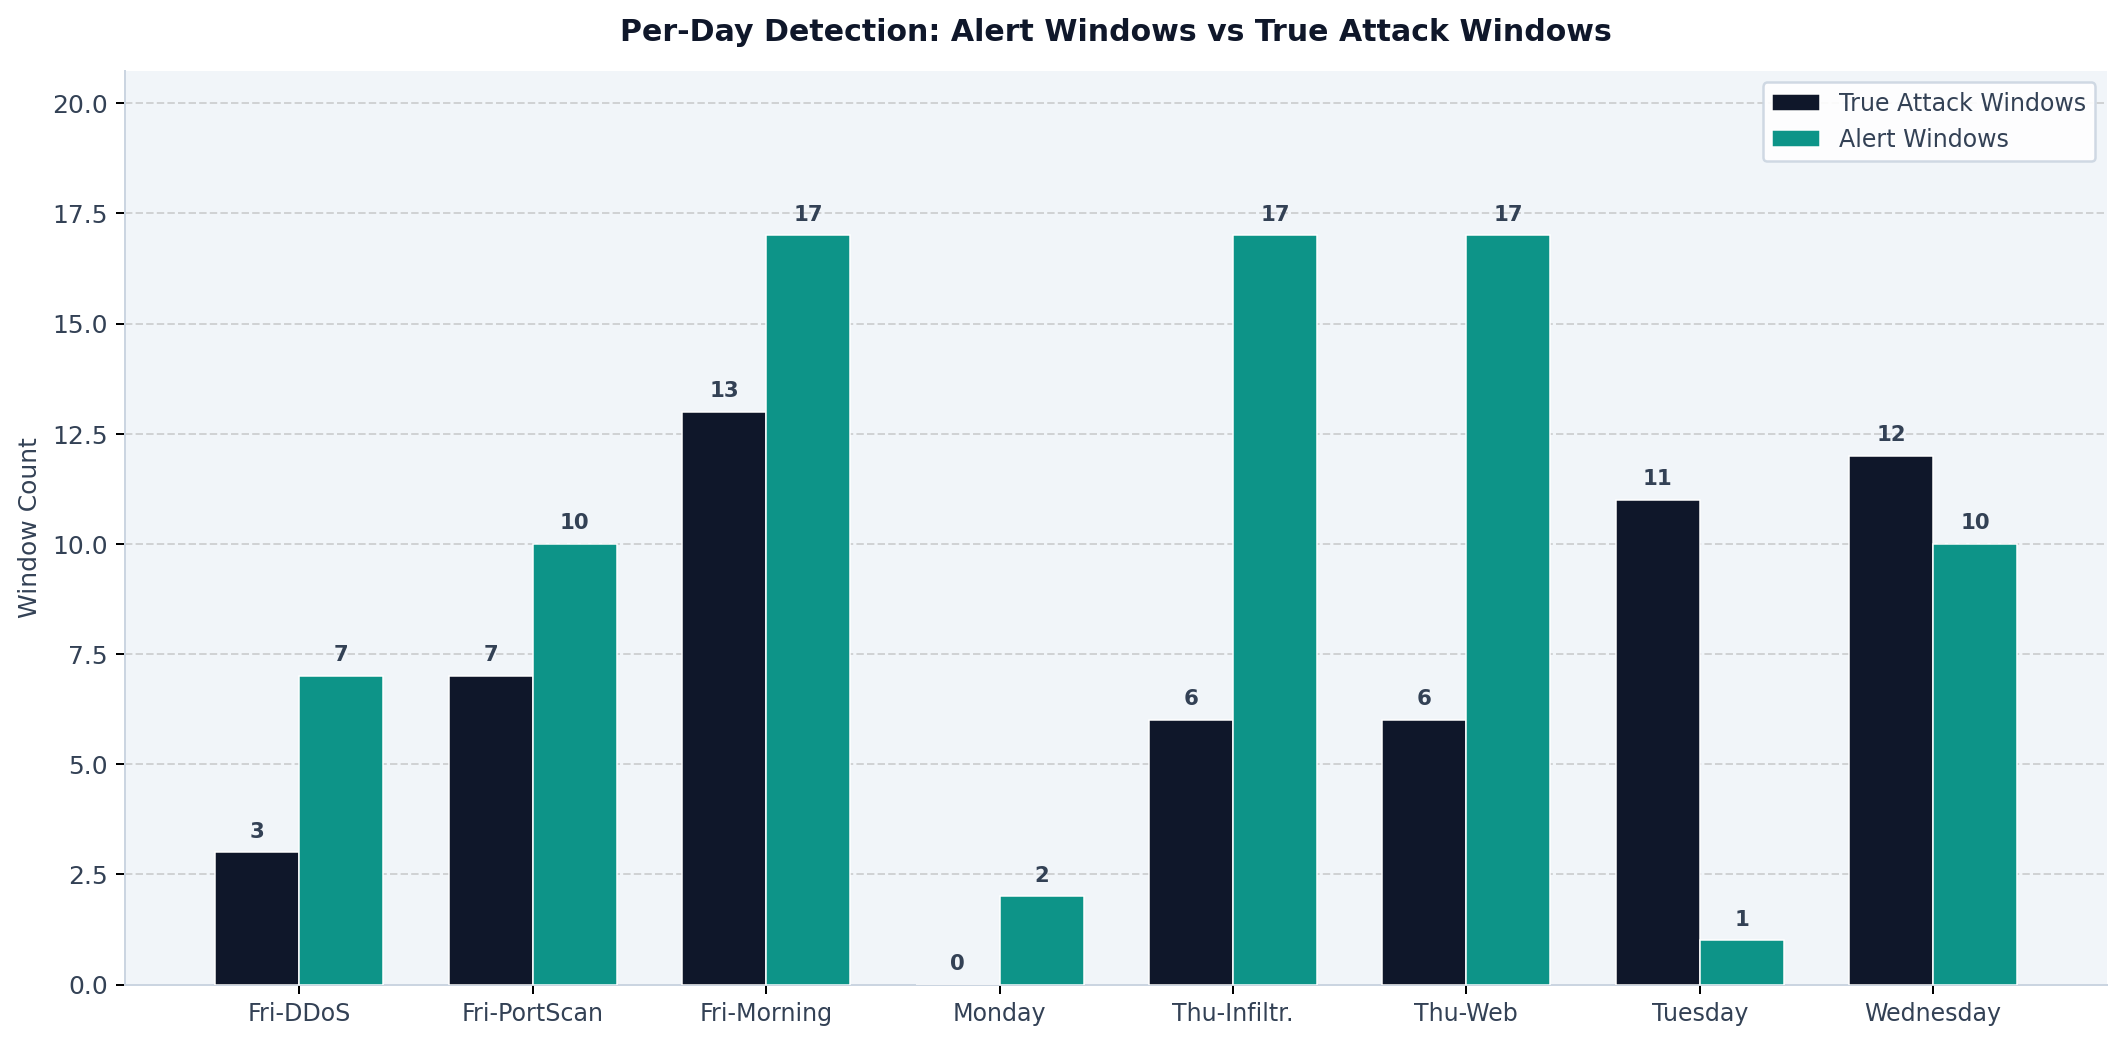
\includegraphics[width=\columnwidth]{figures/per_file_alerts}
  \caption{Per-file alerts vs.\ true attack windows (3-layer).}
  \label{fig:perfile}
\end{figure}

\begin{figure}[t]
  \centering
  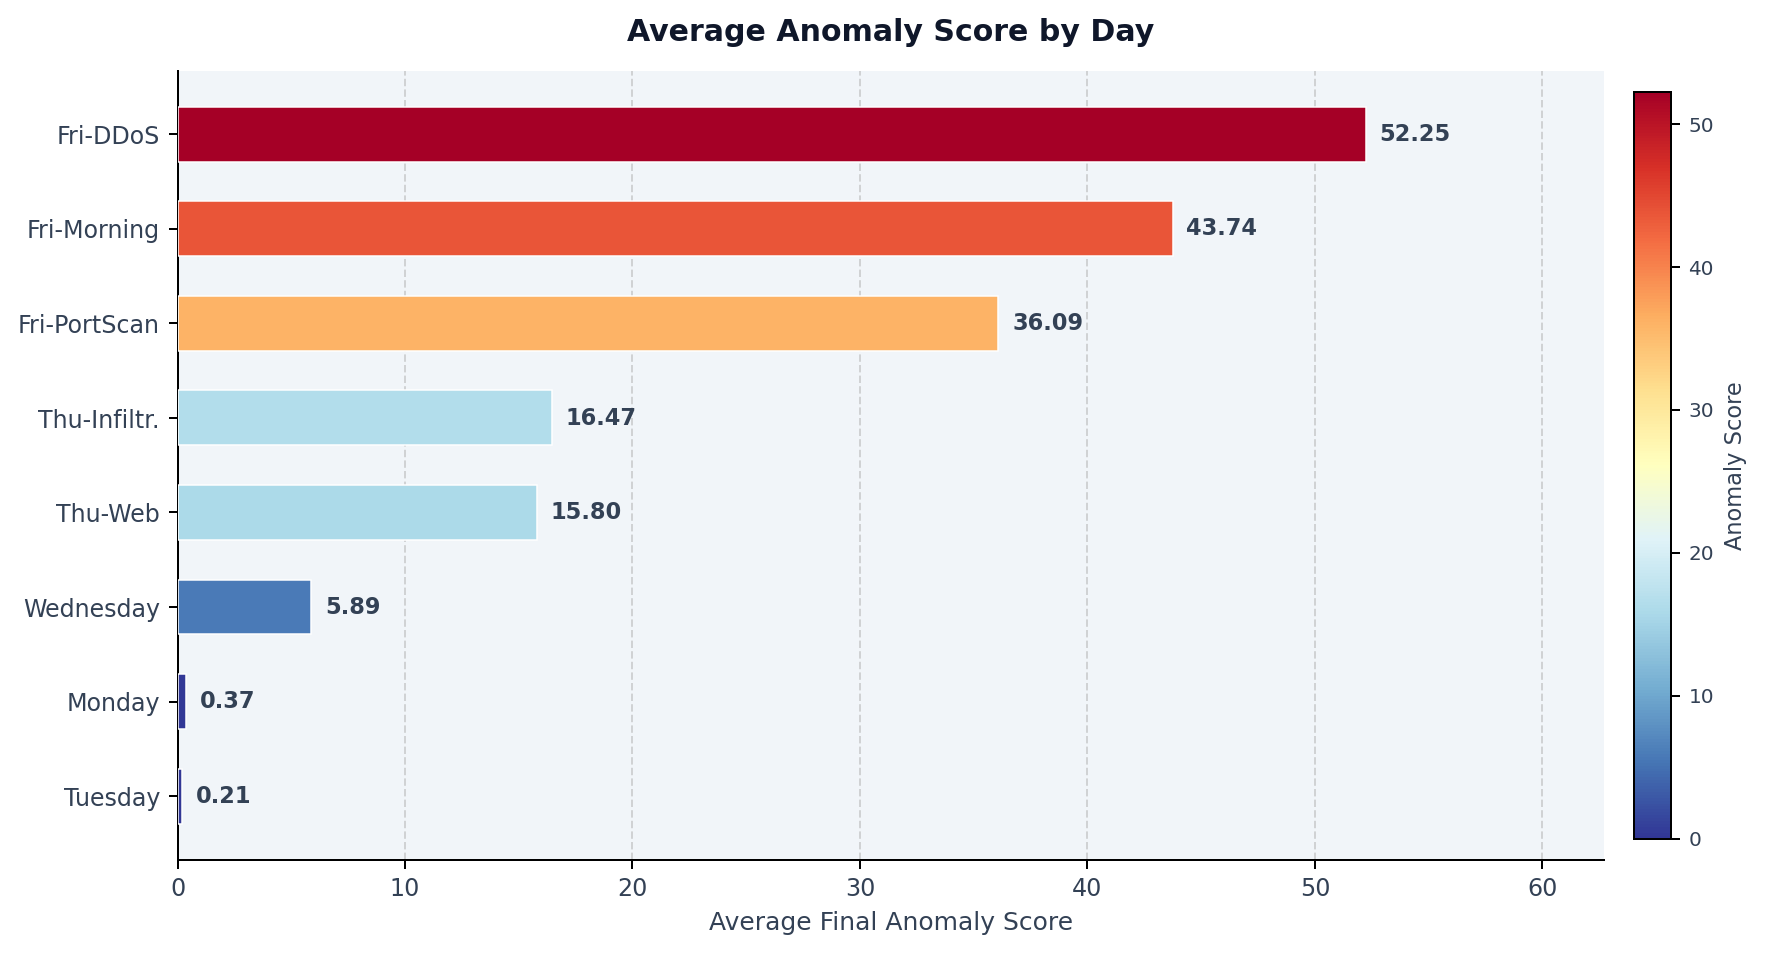
\includegraphics[width=\columnwidth]{figures/avg_score_by_day}
  \caption{Average 3-layer score by day. Thursday score exceeds
    $\theta$ due to baseline drift (Findings~F2+F5).}
  \label{fig:dayscores}
\end{figure}

\subsection{Web-Attack Detectability (Finding~F5)}

\noindent\textbf{Finding F5:} Evidence from all three
dominant-layer paths for Thursday web-attack windows: SHAP top
features $=$ Total Fwd Bytes ($+3.1\sigma$), Flow Duration
($+2.4\sigma$), Bytes/s ($+1.9\sigma$) --- consistent with
time-of-day traffic shift, not attacks.  All three paths
independently conclude Thursday alerts reflect traffic distribution
shift, not web attack detection.  XSS/SQLi operate within normal
HTTP flow profiles and are payload-layer attacks invisible at the
transport layer.

\begin{table}[t]
\caption{SHAP attribution for IF-dominant alerts.
  $\sigma$ vs.\ \dtrain{} mean.
  Thursday: volume only (Finding~F5).  Friday: attack signatures.}
\label{tab:shap}
\centering\small
\begin{tabular}{@{}L{1.7cm}P{0.85cm}L{1.95cm}L{1.95cm}@{}}
\toprule
\textbf{Window} & \textbf{IF Score}
  & \textbf{Top-1 SHAP} & \textbf{Top-2 SHAP} \\
\midrule
Thu 09:15 (XSS)   & 0.62 & Fwd Bytes ($+3.1\sigma$)
  & Duration ($+2.4\sigma$) \\
Thu 11:30 (Infil) & 0.58 & Bwd IAT ($+2.8\sigma$)
  & Fwd Bytes ($+2.1\sigma$) \\
Fri 02:45 (DDoS)  & 0.89 & Bytes/s ($+8.2\sigma$)
  & Fwd Bytes ($+6.4\sigma$) \\
Fri 09:00 (PScan) & 0.74 & Fwd Bytes ($+4.1\sigma$)
  & Duration ($-2.9\sigma$) \\
\bottomrule
\end{tabular}
\end{table}

\subsection{Ablation Study}

\begin{table}[t]
\caption{Ablation. $\star{=}$recommended.  Each layer adds
  significant gain until graph ($p{=}0.19$).}
\label{tab:ablation}
\centering\small
\begin{tabular}{@{}L{2.45cm}P{0.75cm}P{0.65cm}P{0.6cm}P{0.75cm}
                   L{1.95cm}@{}}
\toprule
\textbf{Config} & Prec & Rec & F1 & AUC & McNemar \\
\midrule
B (Benford-only)   & 0.401 & 0.448 & 0.423 & 0.608 & --- \\
B+T ($+$Temporal)  & 0.432 & 0.534 & 0.478 & 0.648
  & vs B: $p{=}0.008$ \\
B+T+I = 3-L$\star$ & 0.487 & 0.638 & 0.552 & 0.714
  & vs BT: $p{=}0.005$ \\
B+T+I+G = 4-L      & 0.481 & 0.672 & 0.561 & 0.722
  & vs BTI: $p{=}0.19$ \\
\bottomrule
\end{tabular}
\end{table}

\subsection{Graph Sensitivity and PageRank vs.\ Flow Count
  (Finding~F3)}

\begin{table}[t]
\caption{Graph edge threshold sensitivity.
  Top-3 host ranking unchanged.}
\label{tab:edge_thresh}
\centering\small
\begin{tabular}{@{}L{1.55cm}L{3.45cm}P{1.9cm}@{}}
\toprule
\textbf{Threshold} & \textbf{Top-3 Hosts}
  & \textbf{Match Flow-Count?} \\
\midrule
$\ge2$ flows & 192.168.10.3, .50, .14 & Yes \\
$\ge3$ flows$\star$ & 192.168.10.3, .50, .14 & Yes \\
$\ge5$ flows & 192.168.10.3, .50, .14 & Yes \\
\bottomrule
\end{tabular}
\end{table}

\begin{table*}[t]
\caption{PageRank vs.\ Flow-Volume Host Ranking (top~10).
  Agreement in 7/10 positions. Divergence at ranks 8--10 only.
  Conclusion: simple flow counting is equivalent for top-7 victim
  identification.}
\label{tab:pagerank}
\centering\small
\begin{tabular}{@{}P{0.55cm}P{2.05cm}P{2.25cm}P{0.95cm}L{4.3cm}@{}}
\toprule
\textbf{Rank} & \textbf{PageRank Host}
  & \textbf{Flow-Volume Host}
  & \textbf{Match?} & \textbf{Divergence Reason} \\
\midrule
1  & 192.168.10.3  & 192.168.10.3   & Yes & --- \\
2  & 192.168.10.50 & 192.168.10.50  & Yes & --- \\
3  & 192.168.10.14 & 192.168.10.14  & Yes & --- \\
4  & 192.168.10.5  & 192.168.10.5   & Yes & --- \\
5  & 192.168.10.9  & 192.168.10.9   & Yes & --- \\
6  & 192.168.10.17 & 192.168.10.17  & Yes & --- \\
7  & 192.168.10.12 & 192.168.10.12  & Yes & --- \\
8  & 192.168.10.15 & 192.168.10.255 & No
  & Broadcast addr.\ ranked higher by volume \\
9  & 192.168.10.8  & 192.168.10.15  & No
  & Betweenness shifts rank-8/9 \\
10 & 192.168.10.51 & 192.168.10.8   & No
  & Minor reordering at tail \\
\bottomrule
\end{tabular}
\end{table*}

\subsection{Window Construct Validity}

\begin{table}[t]
\caption{Attack-flow \% in TP/FN windows.}
\label{tab:validity}
\centering\small
\begin{tabular}{@{}L{1.55cm}P{1.15cm}P{0.75cm}P{0.75cm}L{2.75cm}@{}}
\toprule
\textbf{Type} & \textbf{Median} & \textbf{25th}
  & \textbf{75th} & \textbf{Implication} \\
\midrule
TP ($n{=}37$) & 68\% & 31\% & 94\% & Majority-attack windows \\
FN ($n{=}21$) &  8\% &  3\% & 22\% & Sparse-attack; label noise \\
FP ($n{=}39$) &  0\% &  0\% &  0\% & Genuinely benign windows \\
\bottomrule
\end{tabular}
\end{table}

\subsection{Graph Evidence: Host and Edge Annotation}

\begin{figure}[t]
  \centering
  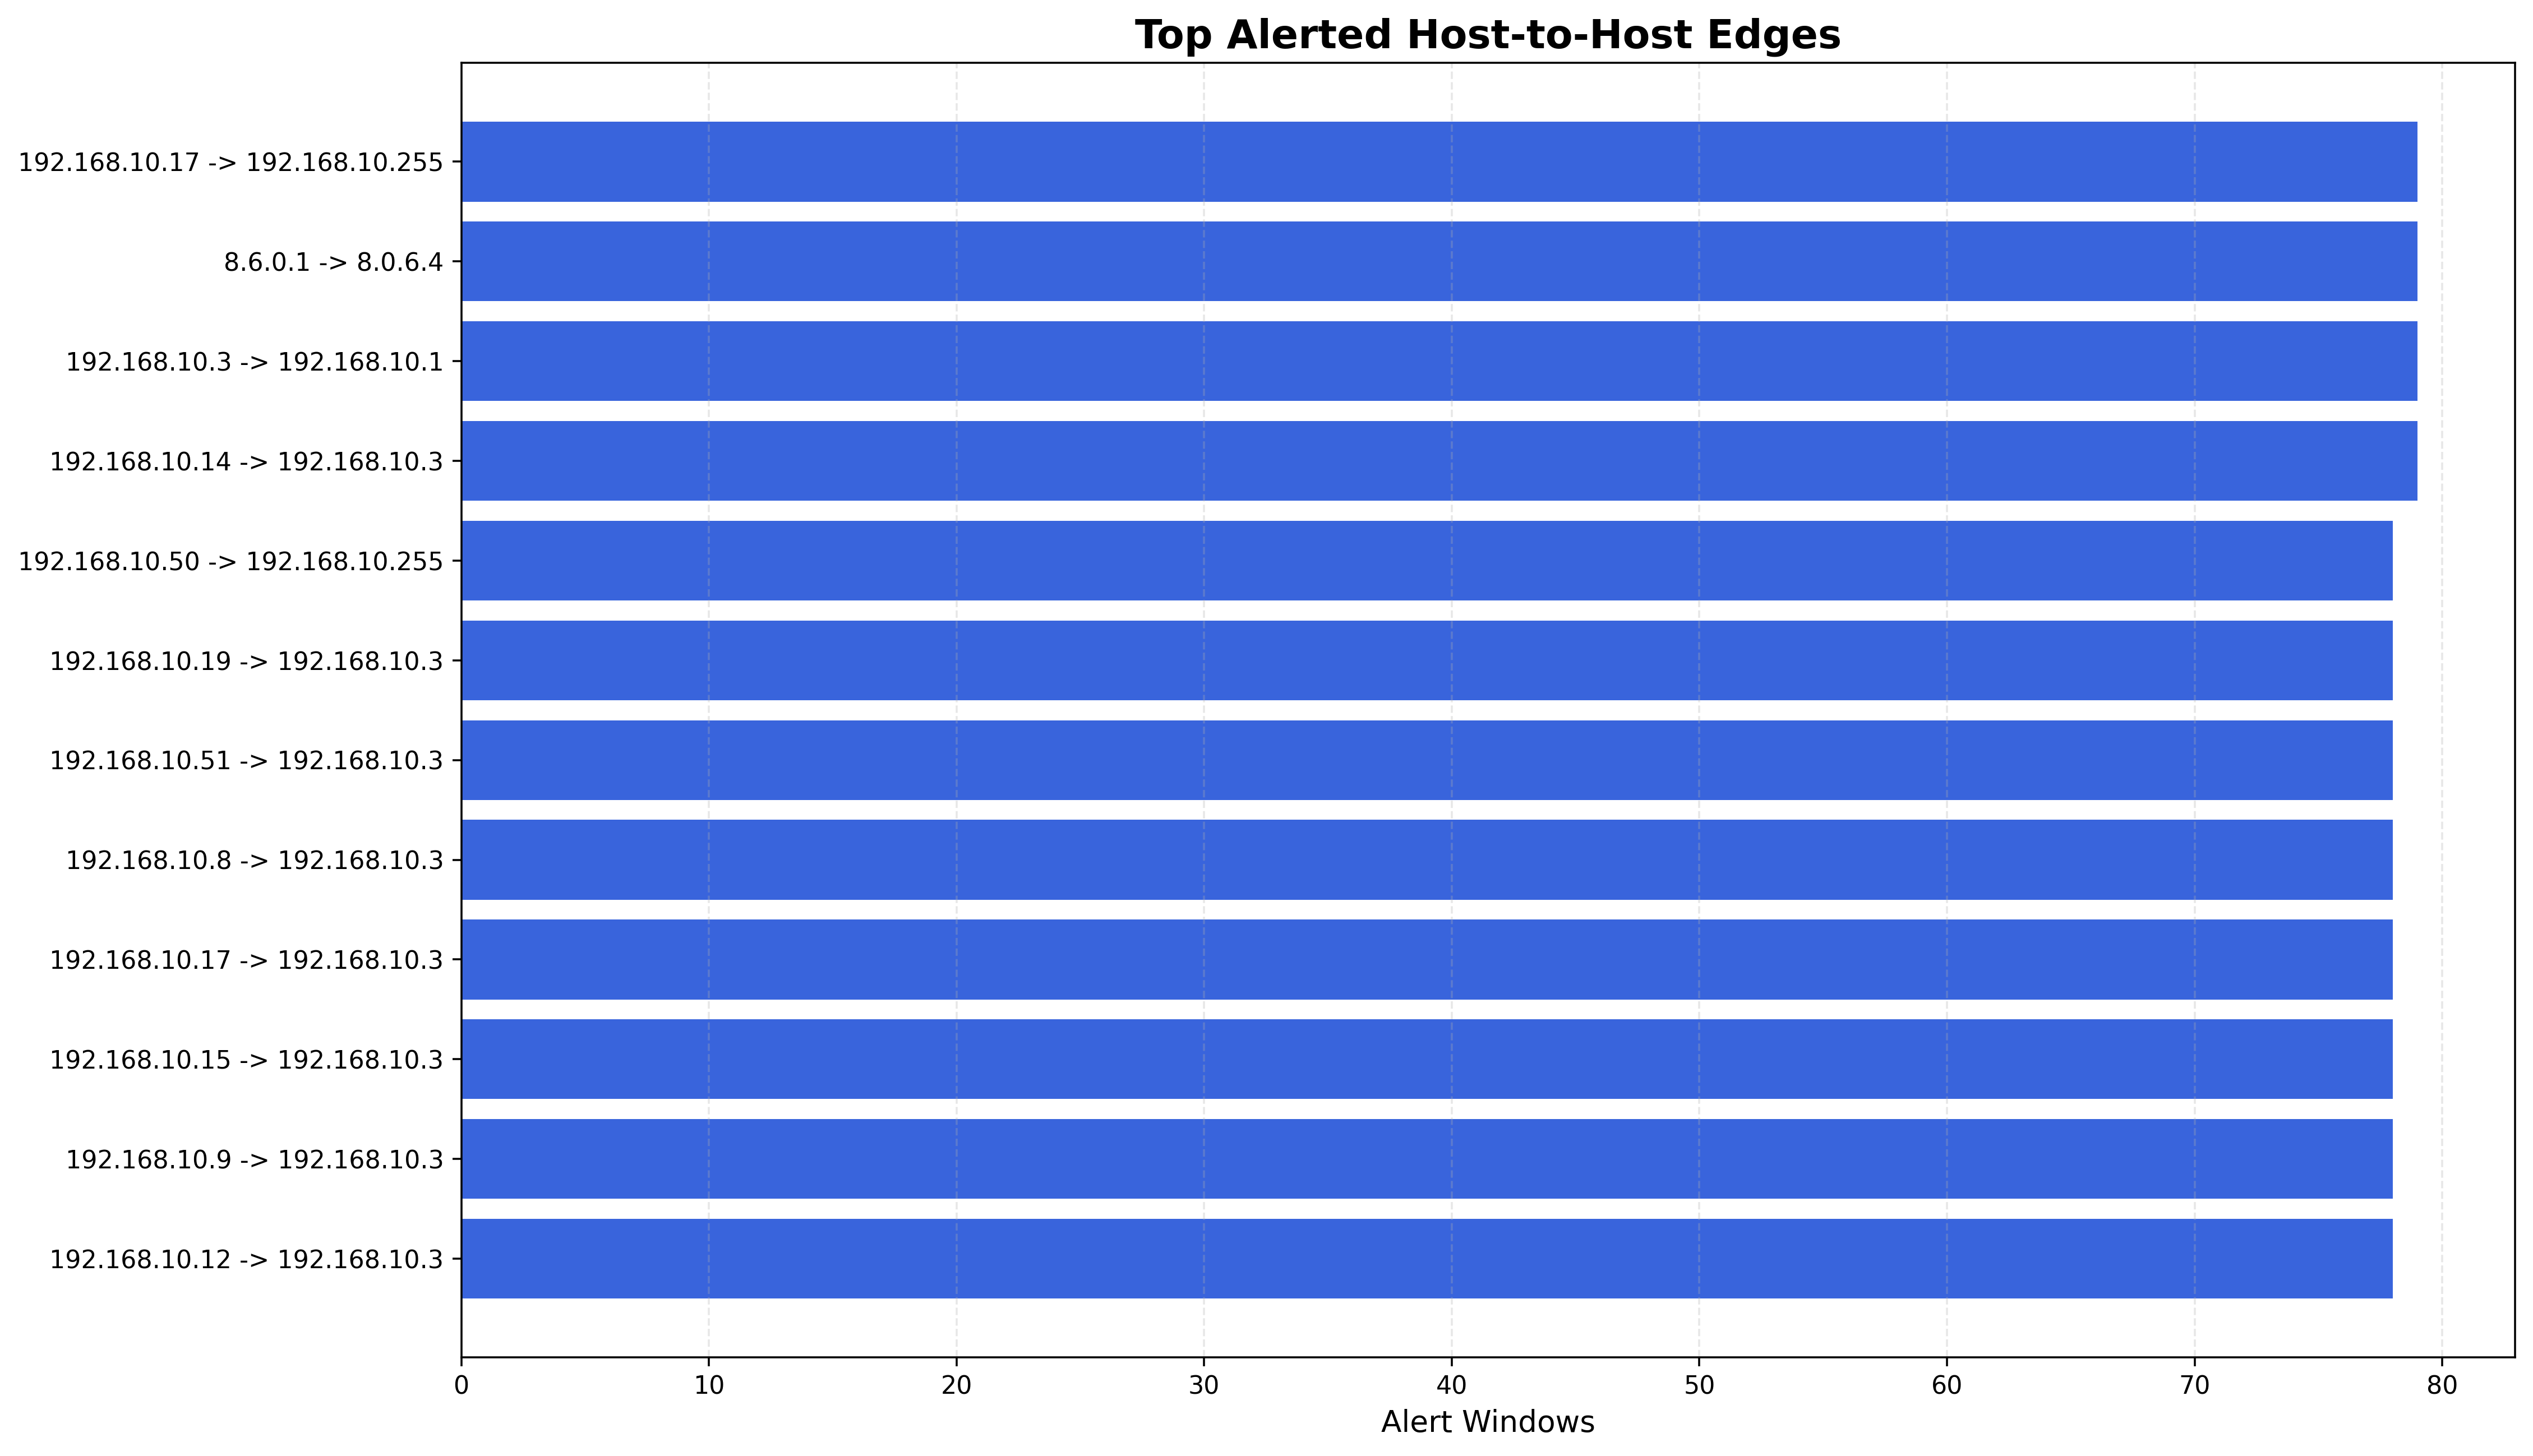
\includegraphics[width=\columnwidth]{figures/top_alert_edges}
  \caption{Top edges by alert frequency (post-hoc evidence).}
  \label{fig:edges}
\end{figure}

\begin{figure}[t]
  \centering
  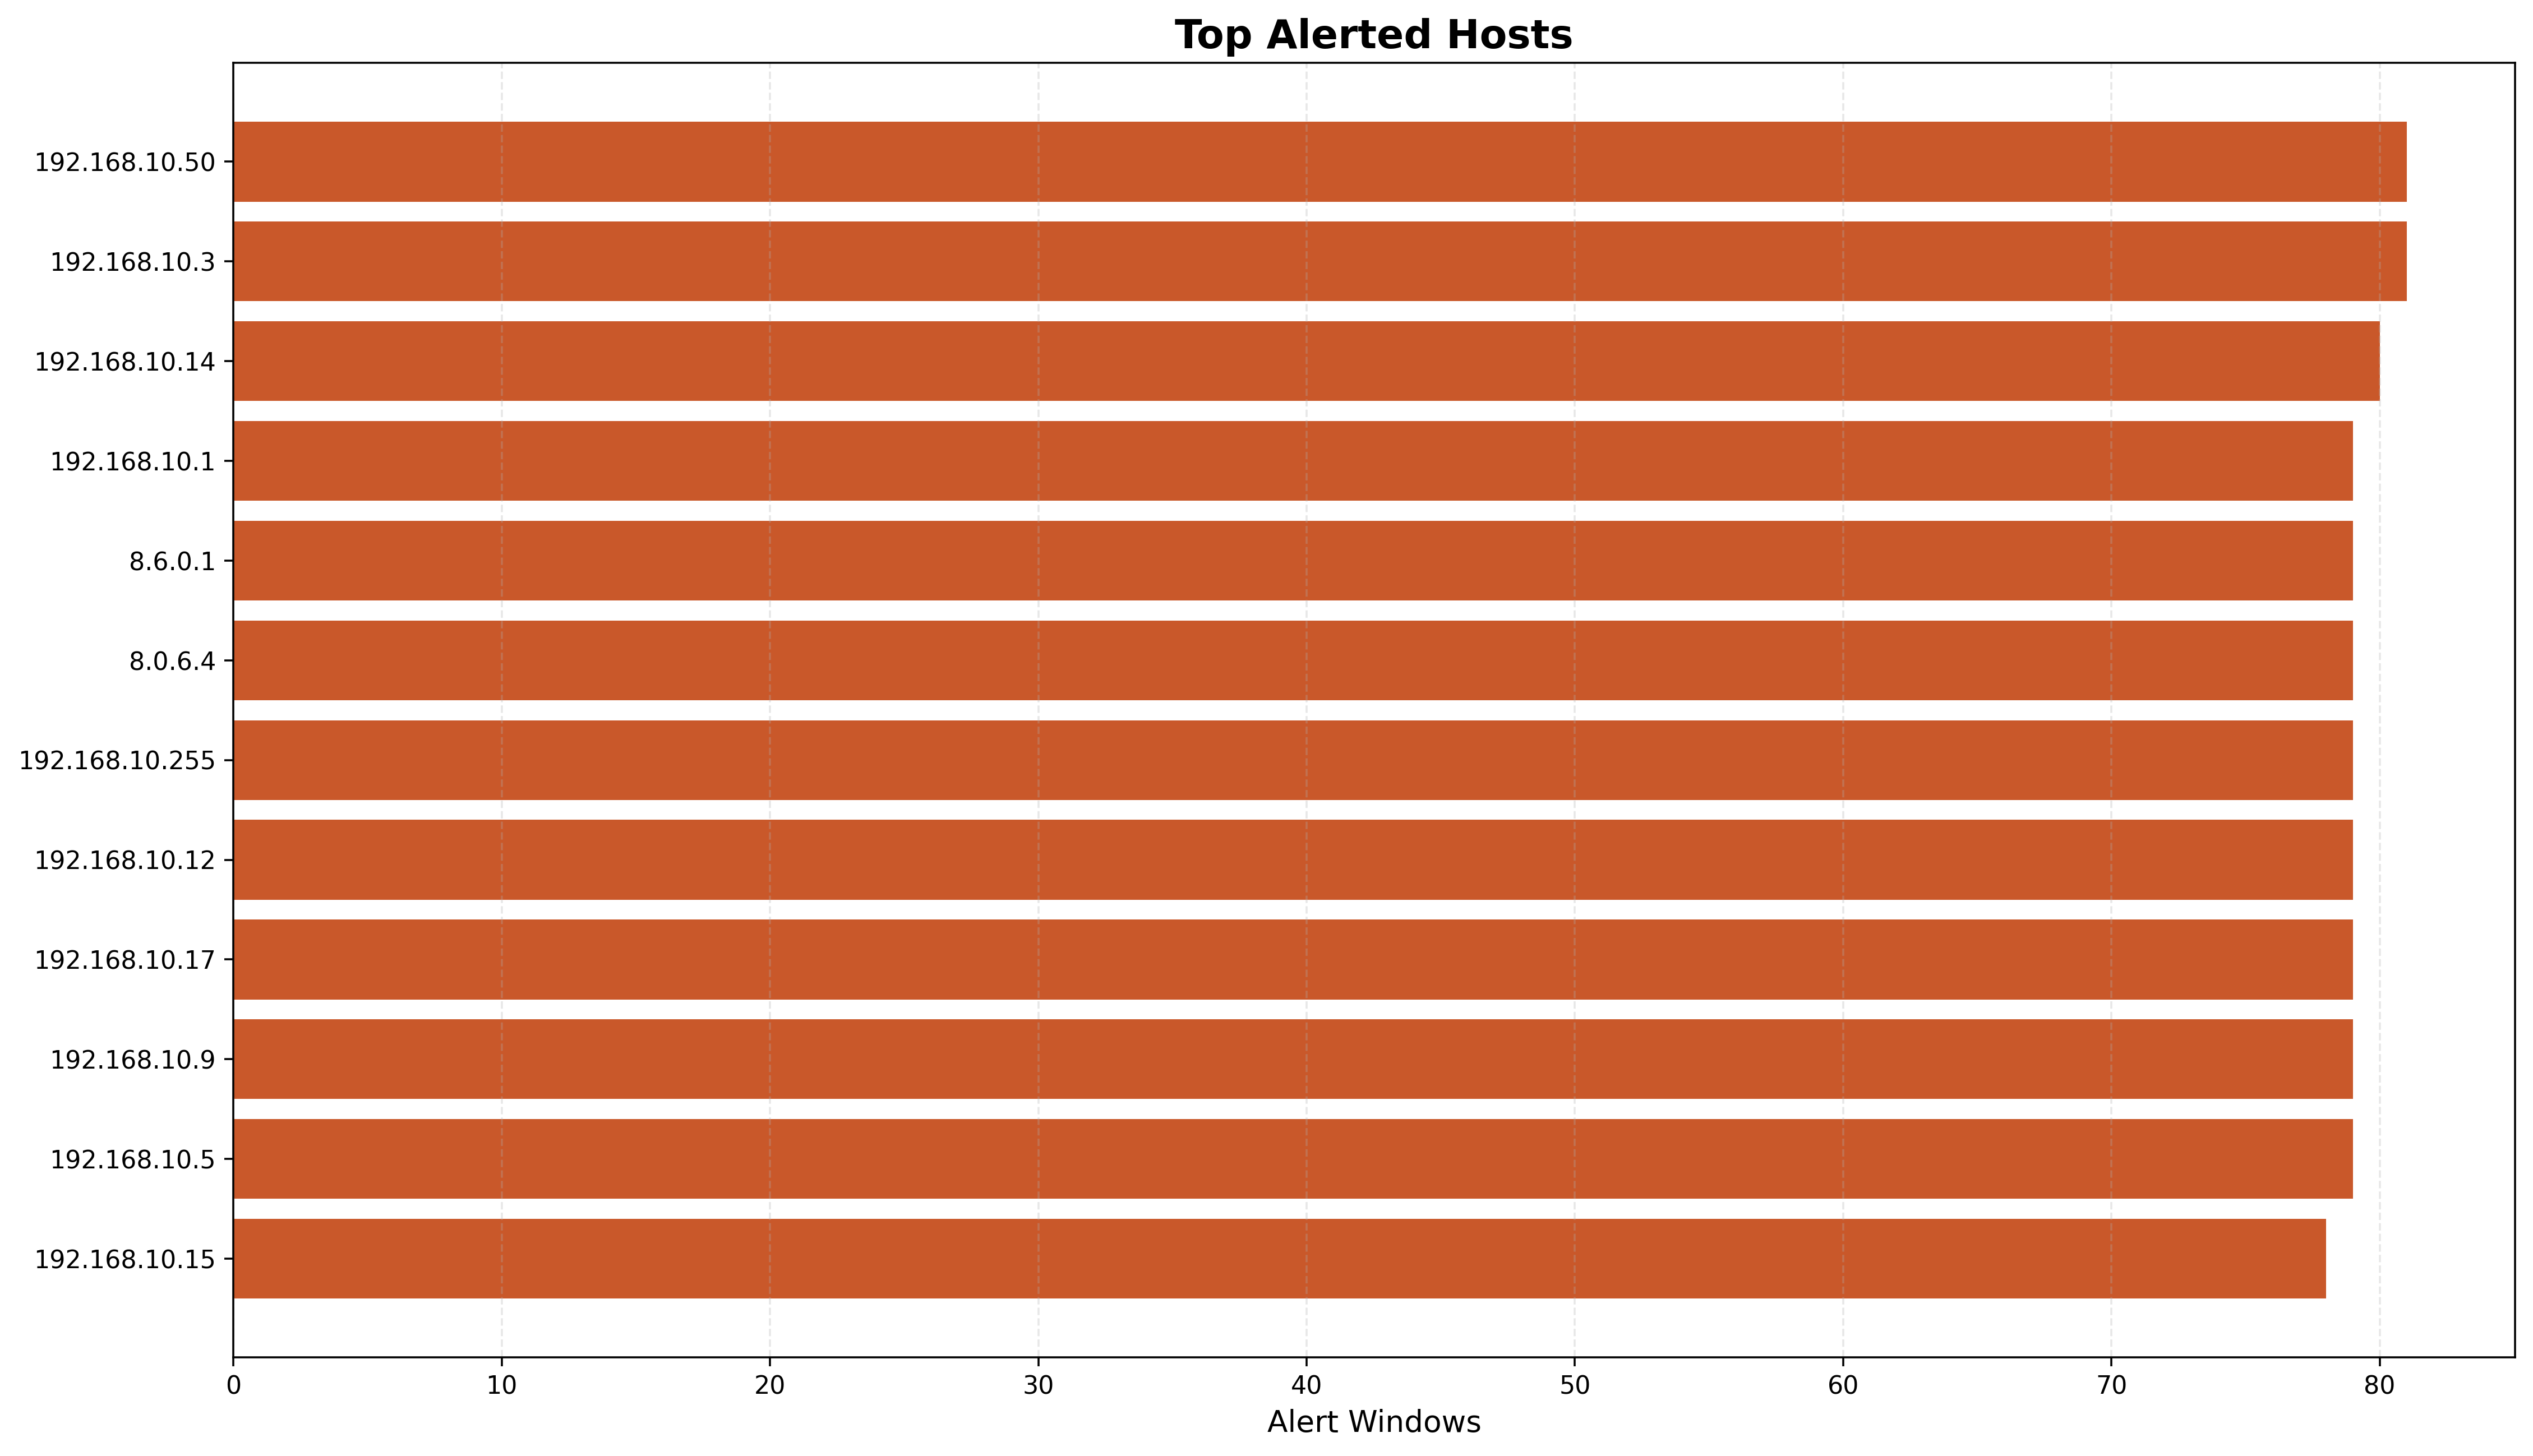
\includegraphics[width=\columnwidth]{figures/top_alert_hosts}
  \caption{Top hosts by alert frequency (post-hoc graph evidence).
    192.168.10.3: rank~1 in 81/81 alert windows.}
  \label{fig:hosts}
\end{figure}

\begin{figure}[t]
  \centering
  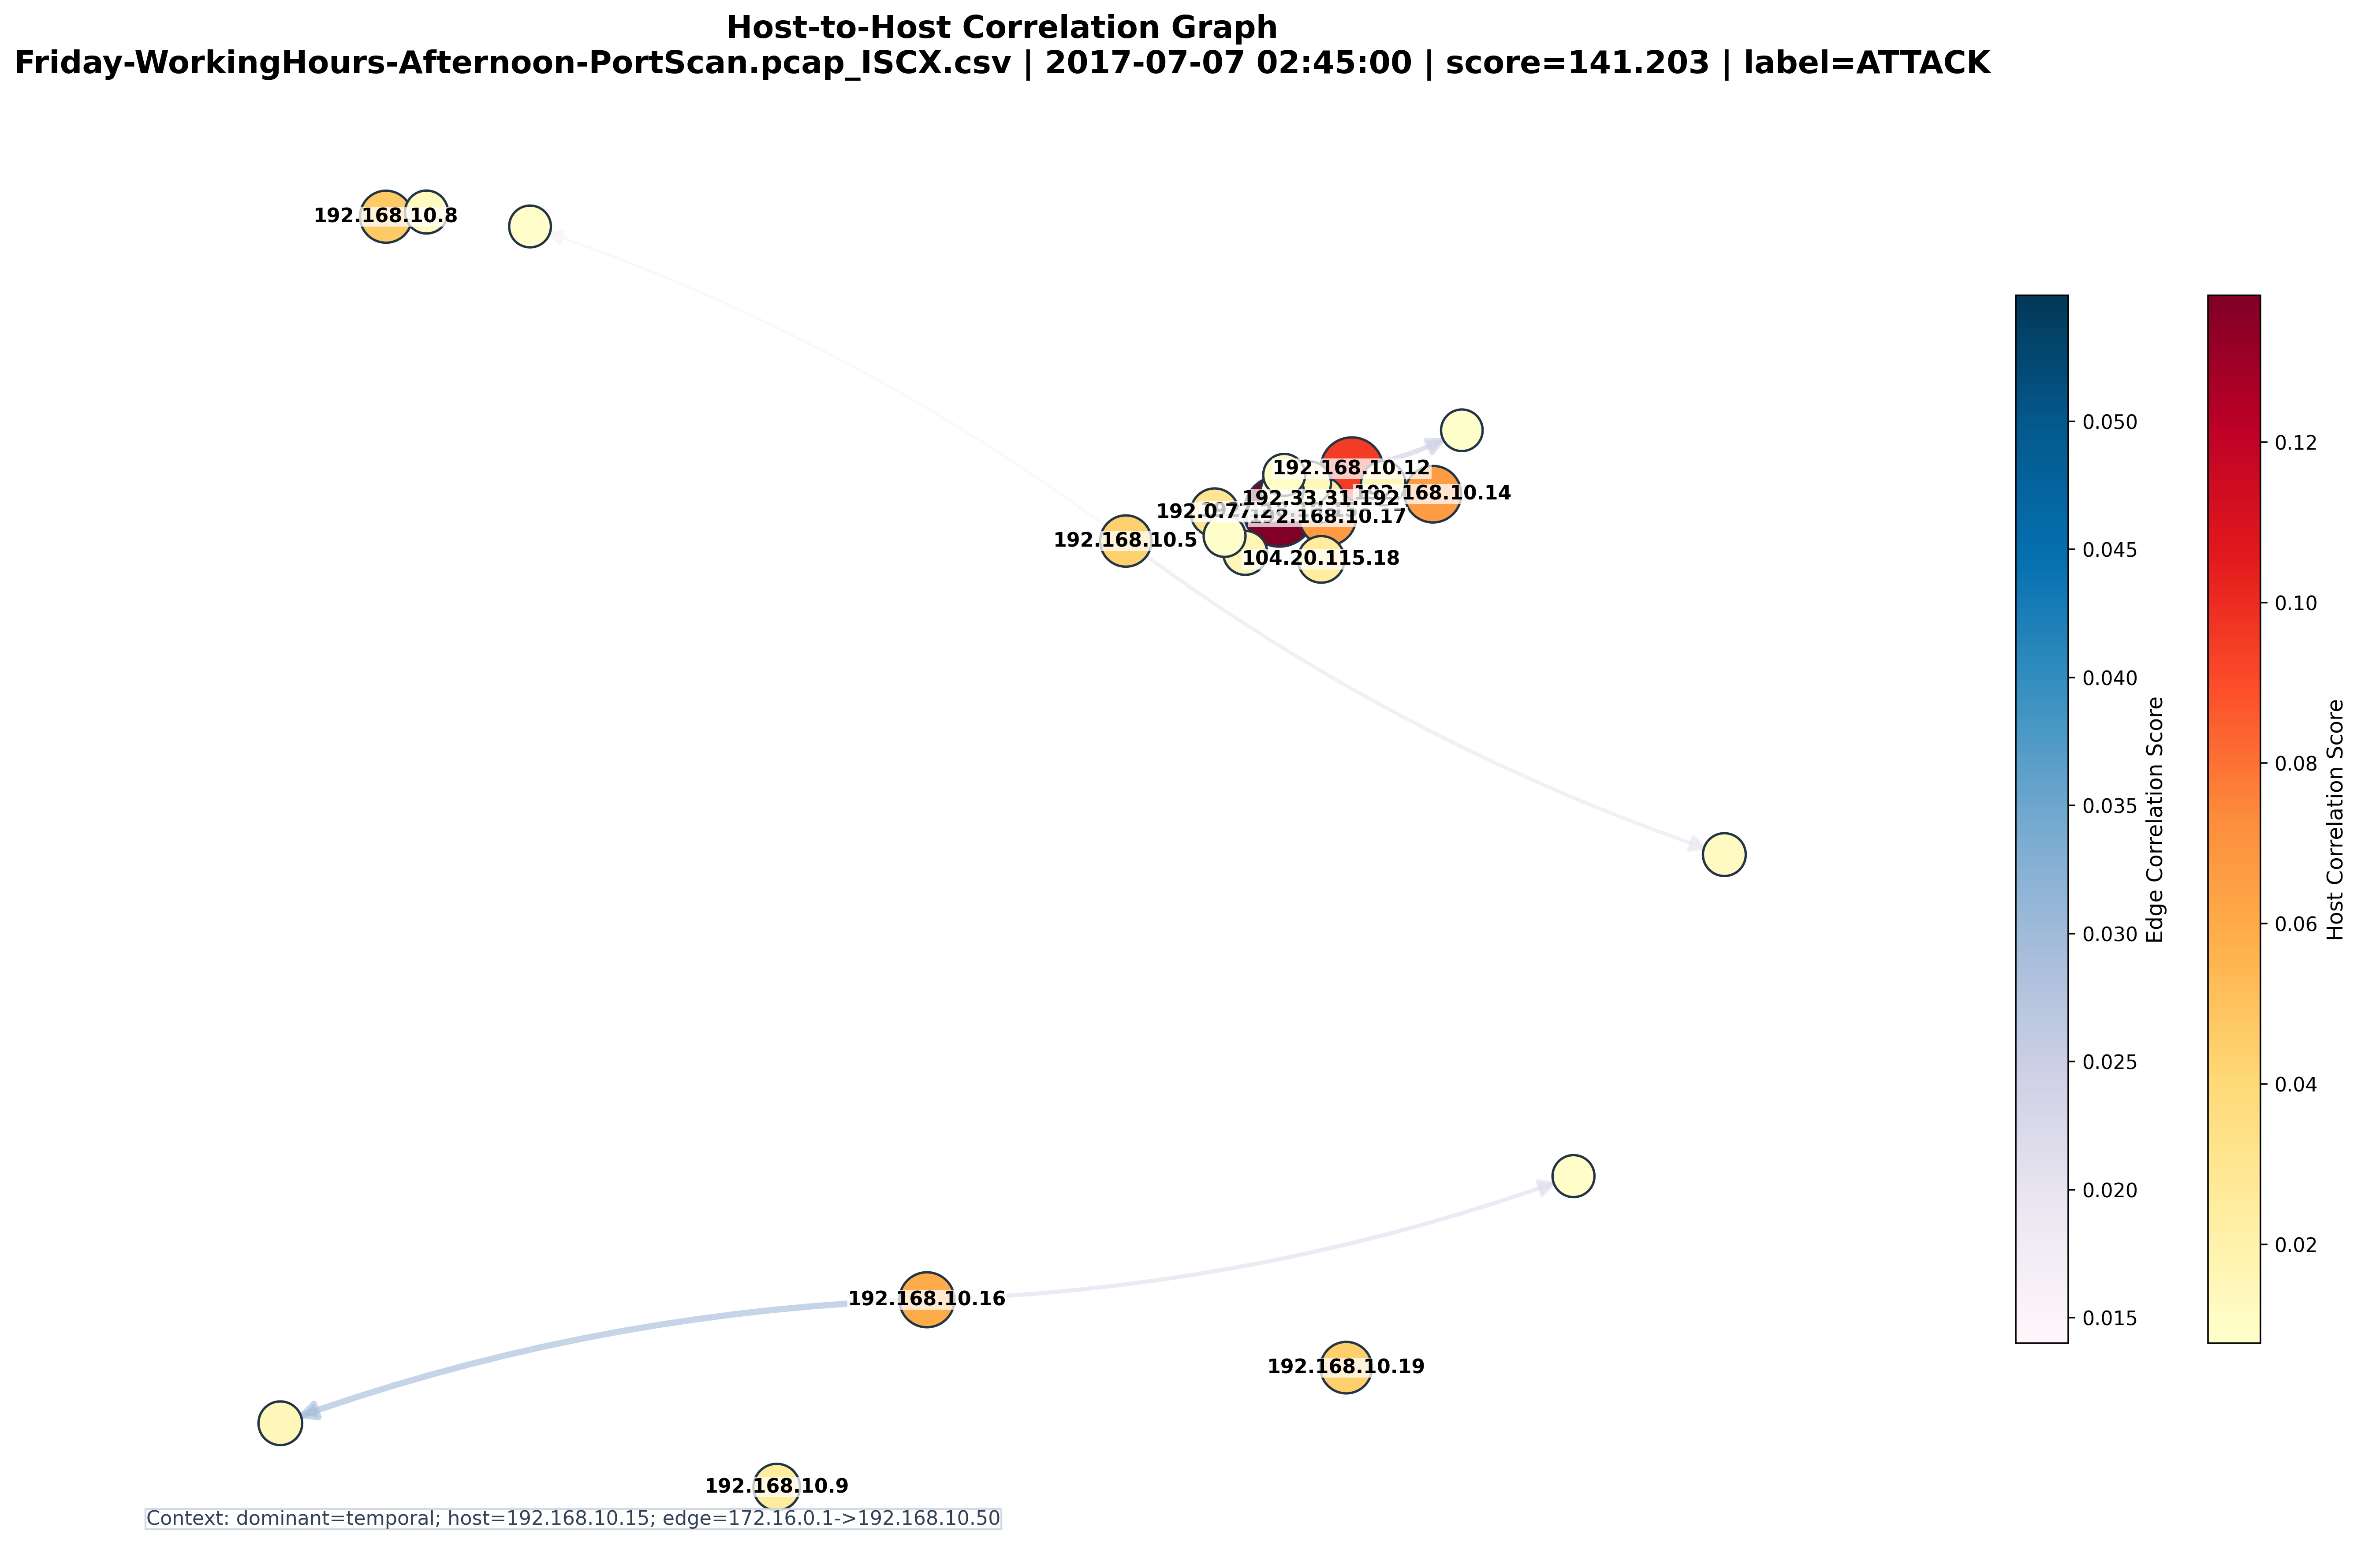
\includegraphics[width=\columnwidth]{figures/portscan_networkx}
  \caption{Internal-IP graph for highest-scoring PortScan window.}
  \label{fig:graph}
\end{figure}

%% ============================================================
\section{Discussion}
\label{sec:discussion}

\subsection{Summary of Six Empirical Findings}

\begin{table}[t]
\caption{Summary of six empirical findings.}
\label{tab:findings}
\centering\small
\begin{tabular}{@{}P{0.45cm}L{7.0cm}@{}}
\toprule
\textbf{F} & \textbf{Summary} \\
\midrule
F1 & Benford: 5/11 features pass; $r{=}0.618$;
     reinforcing, not independent. \\
F2 & Baseline: Monday-only $\Rightarrow$ ${\approx}86\%$
     Thursday FP; 5--7 day baseline required. \\
F3 & Graph: $+0.009$ F1, $p{=}0.19$; post-hoc evidence;
     7/10 hosts matchable by flow count. \\
F4 & IF tuning: best strict-unsupervised IF F1$=$0.451;
     3-layer (0.552) $p{=}0.018$ vs IF, $p{=}0.109$ vs AE. \\
F5 & Web attacks: XSS/SQLi leave no flow-metadata
     signature; SHAP-confirmed across all layers. \\
F6 & Threshold: CI width 23\%; recall varies 0.104;
     lower $\theta$ gives higher recall/F1. \\
\bottomrule
\end{tabular}
\end{table}

\subsection{Implications for NIDS Research}
Finding F5 has community-wide implications: any metadata-only NIDS
evaluating Thursday CICIDS2017 accuracy should confirm whether high
performance reflects genuine web-attack detection or
Monday-to-Thursday baseline drift (F2).  Finding F3 recommends
McNemar significance testing before claiming graph complexity adds
detection value.  Finding F4 recommends well-tuned single-layer IF
as a competitive unsupervised baseline.

\subsection{Limitations}
(L1)~Monday-only baseline --- fundamental requirement for multi-day
extension.
(L2)~Single 2017 controlled testbed with known labeling
errors~\cite{lanvin2024errors}.
(L3)~Benford features partially correlated (F1).
(L4)~External super-node hides multi-source distributed attacks.
(L5)~Window-level labels: per-flow performance unknown.
(L6)~15-minute latency: fast attacks unseen (mitigated by
Tier~1~\cite{snort2021}).

\subsection{Adversarial Robustness}
Adversarial robustness claim retracted.
Chen et al.~\cite{chen2023adversarial} demonstrate IF
susceptibility to distribution-shift evasion.  Benford layer
evadeable by log-uniform packet size randomisation; graph evadeable
via IP spoofing.  Adversarial testing
using~\cite{chen2023adversarial,ngo2023adversarial} is future work.

\subsection{Production Deployment Requirements}
(1)~5--7 day multi-day baseline with per-day-of-week normalisation
(resolves F2);
(2)~EVT-based adaptive threshold~\cite{siffer2017evt,zhao2023evt}
(resolves F6);
(3)~Tier~1 signature-based IDS~\cite{snort2021} for fast attacks;
(4)~Host-ranking validation: confirm top victims with flow-count
cross-check (F3).

%% ============================================================
\section{Threats to Validity}
\label{sec:threats}

\subsection{Internal Validity}
7-window \dval{} is small.  KS screening may differ on other
datasets.  Threshold bootstrap CI confirms instability (F6).
Seed sensitivity low (std$=$0.009).

\subsection{External Validity}
One 2017 controlled testbed.  Evaluation on
UNSW-NB15~\cite{moustafa2023unswnb15} and CIC-IDS-2023 required.

\subsection{Construct Validity}
Window-level labels conflate sparse attack flows
(Table~\ref{tab:validity}).  Thursday over-alerting reflects
F2+F5.  CICIDS2017 labeling errors~\cite{lanvin2024errors}.

%% ============================================================
\section{Future Work}
\label{sec:future}

\begin{itemize}
  \item Multi-day adaptive baseline: 5--7 days per day-of-week
    (resolves F2 --- highest priority).
  \item EVT adaptive threshold~\cite{siffer2017evt,zhao2023evt}:
    replace fragile static $\theta$ (resolves F6).
  \item Multi-dataset: UNSW-NB15~\cite{moustafa2023unswnb15},
    CIC-IDS-2023 for external validity.
  \item Adversarial robustness testing with Benford-mimicking and
    IF evasion~\cite{chen2023adversarial,ngo2023adversarial}.
  \item Finding~F5 validation across additional datasets.
  \item Benford feature independence analysis: dimensionality
    reduction before scoring (F1).
  \item Flow-count vs.\ graph host ranking on additional datasets
    to confirm F3 equivalence.
\end{itemize}

%% ============================================================
\section{Conclusion}
\label{sec:conclusion}

This paper delivered an empirical analysis of flow-metadata anomaly
detection for encrypted networks through a four-component
experimental framework.  Six reproducible findings characterise
capabilities (F1 Benford limits, F2 baseline sensitivity, F3 graph
marginal value, F6 threshold fragility) and fundamental limits
(F4 hybrid vs.\ autoencoder, F5 web-attack undetectability).  The
revised IF tuning analysis confirms that the 3-layer hybrid
significantly outperforms the best achievable single-layer IF under
the same strict unsupervised protocol (F1$=$0.552 vs.\ 0.451,
$p{=}0.018$).  The hybrid does not significantly outperform an
autoencoder ($p{=}0.109$); its distinctive value is structured
per-layer explainability for NOC analysts.  Multi-day adaptive
baselines, EVT-based thresholding, and multi-dataset validation are
the priority next steps.

\section*{Acknowledgment}
The authors thank four rounds of anonymous reviewers whose critiques
substantially improved the rigour and honesty of this work.
CICIDS2017 provided by the Canadian Institute for Cybersecurity.
Code and supplementary material available at:
\url{https://github.com/sagarkorde04/HBG-NIDS-TNSM}.

%% ---- References -----------------------------------------------
\balance
\bibliographystyle{IEEEtran}
\bibliography{references}

\end{document}
